%%% Hlavní soubor. Zde se definují základní parametry a odkazuje se na ostatní části. %%%

%% Verze pro jednostranný tisk:
% Okraje: levý 40mm, pravý 25mm, horní a dolní 25mm
% (ale pozor, LaTeX si sám přidává 1in)
\documentclass[12pt,a4paper]{report}
\setlength\textwidth{145mm}
\setlength\textheight{247mm}
\setlength\oddsidemargin{15mm}
\setlength\evensidemargin{15mm}
\setlength\topmargin{0mm}
\setlength\headsep{0mm}
\setlength\headheight{0mm}
% \openright zařídí, aby následující text začínal na pravé straně knihy
\let\openright=\clearpage

\setcounter{secnumdepth}{3}

%% Pokud tiskneme oboustranně:
% \documentclass[12pt,a4paper,twoside,openright]{report}
% \setlength\textwidth{145mm}
% \setlength\textheight{247mm}
% \setlength\oddsidemargin{14.2mm}
% \setlength\evensidemargin{0mm}
% \setlength\topmargin{0mm}
% \setlength\headsep{0mm}
% \setlength\headheight{0mm}
% \let\openright=\cleardoublepage

%% Vytváříme PDF/A-2u
\usepackage[a-2u]{pdfx}

%% Přepneme na českou sazbu a fonty Latin Modern
\usepackage[czech]{babel}
\usepackage{lmodern}
\usepackage[T1]{fontenc}
\usepackage{textcomp}

%% Použité kódování znaků: obvykle latin2, cp1250 nebo utf8:
\usepackage[utf8]{inputenc}

%%% Další užitečné balíčky (jsou součástí běžných distribucí LaTeXu)
\usepackage{amsmath}        % rozšíření pro sazbu matematiky
\usepackage{amsfonts}       % matematické fonty
\usepackage{amsthm}         % sazba vět, definic apod.
\usepackage{bbding}         % balíček s nejrůznějšími symboly
			    % (čtverečky, hvězdičky, tužtičky, nůžtičky, ...)
\usepackage{bm}             % tučné symboly (příkaz \bm)
\usepackage{graphicx}       % vkládání obrázků
\usepackage{fancyvrb}       % vylepšené prostředí pro strojové písmo
\usepackage{indentfirst}    % zavede odsazení 1. odstavce kapitoly
\usepackage{natbib}         % zajištuje možnost odkazovat na literaturu
			    % stylem AUTOR (ROK), resp. AUTOR [ČÍSLO]
\usepackage[nottoc]{tocbibind} % zajistí přidání seznamu literatury,
                            % obrázků a tabulek do obsahu
\usepackage{icomma}         % inteligetní čárka v matematickém módu
\usepackage{dcolumn}        % lepší zarovnání sloupců v tabulkách
\usepackage{booktabs}       % lepší vodorovné linky v tabulkách
\usepackage{paralist}       % lepší enumerate a itemize
\usepackage{xcolor}         % barevná sazba

%%% Údaje o práci

% Název práce v jazyce práce (přesně podle zadání)
\def\NazevPrace{Evoluce robotů v simulovaném\vspace{12pt} fyzikálním prostředí}

% Název práce v angličtině
\def\NazevPraceEN{Evolution of robots in a simulated physical environment}

% Jméno autora
\def\AutorPrace{Marek Bečvář}

% Rok odevzdání
\def\RokOdevzdani{2023}

% Název katedry nebo ústavu, kde byla práce oficiálně zadána
% (dle Organizační struktury MFF UK, případně plný název pracoviště mimo MFF)
\def\Katedra{Katedra softwaru a výuky informatiky}
\def\KatedraEN{Department of software and computer science education}

% Jedná se o katedru (department) nebo o ústav (institute)?
\def\TypPracoviste{Katedra}
\def\TypPracovisteEN{Department}

% Vedoucí práce: Jméno a příjmení s~tituly
\def\Vedouci{RNDr. František Mráz, CSc.}

% Pracoviště vedoucího (opět dle Organizační struktury MFF)
\def\KatedraVedouciho{Katedra softwaru a výuky informatiky}
\def\KatedraVedoucihoEN{Department of software and computer science education}

% Studijní program a obor
\def\StudijniProgram{Informatika}
\def\StudijniObor{Informatika se specializací Umělá inteligence}

% Nepovinné poděkování (vedoucímu práce, konzultantovi, tomu, kdo
% zapůjčil software, literaturu apod.)
\def\Podekovani{%
Rád bych tímto poděkoval panu RNDr. Františku Mrázovi, CSc. za výborné vedení a
aktivní přístup při pravidelných konzultacích, které výrazně přispěly
ke~kvalitě této práce. Zároveň bych chtěl poděkovat mé rodině za nekončící
podporu.
}

% Abstrakt (doporučený rozsah cca 80-200 slov; nejedná se o zadání práce)
\def\Abstrakt{%
Práce představuje systém pro tvorbu a vyhodnocování experimentů s~evolučním
vývojem robotů ve 3D simulovaném fyzikálním prostředí knihovny \emph{MuJoCo}.
Experimenty umožňují vývoj řízení i morfologie robotů za užití libovolné,
uživatelem definované hodnotící funkce. Platforma klade důraz na dostupnost,
čitelnost a rozšiřitelnost implementace. Systém nabízí jednoduché grafické
rozhraní umožňující podrobnou konfiguraci experimentů a~textové rozhraní
vhodné pro provádění rozsáhlých experimentů se statistickým vyhodnocením. Práce
implementuje několik robotů různých složitostí a řadu evolučních algoritmů s
nejznámějšími genetickými operátory. Architektura systému umožňuje při
tvorbě experimentů vytvářet libovolné kombinace těchto prvků. Práce společně s
dokumentací pro uživatele dává jednoduchý návod, jak stávající implementaci
rozšiřovat.
}
\def\AbstraktEN{%
This work introduces a system for designing and evaluating experiments with
evolutionary algorithms in 3D-simulated physical environments of the MuJoCo
library. Experiments allow to develop the control and morphology of robots
while using arbitrary user-defined fitness functions. The implementation was
designed to be as accessible, understandable, and extendable as possible. The
system offers a simple graphical user interface allowing a detailed
configuration of experiments and a text-based user interface which is
convenient for running large amounts of experiments for statistical analysis.
The work implements several robots of different complexity, examples of various
evolutionary algorithms, and a selection of well-known genetic operators.
During experiment design, the architecture of this system allows the combining
of implemented operators and tools arbitrarily. This work and the user
documentation give simple instructions on how to alter and extend the
implementation.
}

% 3 až 5 klíčových slov (doporučeno), každé uzavřeno ve složených závorkách
\def\KlicovaSlova{%
    {evoluční algoritmus}, {robot}, {simulace}
}
\def\KlicovaSlovaEN{%
    {evolutionary algorithm}, {robot}, {simulation}
}

%% Balíček hyperref, kterým jdou vyrábět klikací odkazy v PDF,
%% ale hlavně ho používáme k uložení metadat do PDF (včetně obsahu).
%% Většinu nastavítek přednastaví balíček pdfx.
\hypersetup{unicode}
\hypersetup{breaklinks=true}

%% Definice různých užitečných maker (viz popis uvnitř souboru)
\include{makra}

%% Titulní strana a různé povinné informační strany
\begin{document}
\include{titulka}

%%% Strana s automaticky generovaným obsahem bakalářské práce

\tableofcontents

%%% Jednotlivé kapitoly práce jsou pro přehlednost uloženy v samostatných souborech
\chapter*{Úvod}
\addcontentsline{toc}{chapter}{Úvod}

V dnešní době stále přibývá možností, kde se snažíme aplikovat metody umělé
inteligence pro řešení různorodých problémů. Na řadu z těchto problémů se nám
může nabízet hned několik možných řešení. Problém ale může nastat, pokud si
nejsme jistí, nebo třeba vůbec není možné přesně definovat, co vlastně by mělo
být správným řešením.

\paragraph{}
Pro tyto problémy se nám často hodí využívat metod evolučních algoritmů. Jedná
se o přírodou inspirované optimalizační algoritmy -- konkrétně Darwinovou
evoluční teorií -- které napodobováním přírodních procesů hledají dle našich
požadavků ta nejlepší řešení.

Zacházení s těmito algoritmy ale nemusí být vůbec jednoduché a podobně jako u
dalších optimalizačních metod a metod strojového učení je jejich běh zahalen
množstvím parametrů, které spolu souvisí často špatně předvídatelným způsobem.

\paragraph{}
Z tohoto důvodu je cílem této práce vytvořit platformu, která bude přístupná
uživatelům různých úrovní specializace, umožňující tvořit a provádět
experimenty s evolučními algoritmy. 

S tímto cílem volíme tvořit experimenty s roboty ve virtuálním prostředí,
což~se na tento problém velmi dobře hodí. Uživatel díky robotům intuitivně
chápe složitost problému a každý posun v řešeném problému je interaktivně
pozorovatelný v daném prostředí ještě v průběhu hledání řešení.

Cílem projektu je, aby uživatel dostal kontrolu nad experimenty a mohl tak
získat lepší přehled o práci s evolučními algoritmy a pochopil tak množství
parametrů a jejich vzájemné souvislosti, se kterými se můžeme při tvorbě
experimentů setkat. Projekt bude obsahovat různorodou řadu problémů, na které
bude potřeba využít vícero různých přístupů, což umožní dále rozšířit pochopení
problémů evolučních algoritmů. Nejtěžšími pak mohou být problémy, vyžadující
využití neuronových sítí, což může být pro uživatele díky tomuto projektu
jednoduchým, prvním využitím pokročilého algoritmu pro neuroevoluci (evoluční
vývoj neuronových sítí) -- NEAT.

Pro lehce pokročilého uživatele bude projekt dále nabízet možnosti nahlédnutí
do útrob projektu, prezentující jak se s evolučními algoritmy zachází v
samotném zdrojovém kódu, což mu zároveň umožní tvořit vlastní pokročilé
experimenty a~upravovat a rozšiřovat připravenou databázi částí evolučních
algoritmů o vlastní.

\paragraph{}
Práce je rozdělena do čtyř hlavních kapitol. V kapitole
\ref{chapter-zakladní pojmy} si představíme a~vysvětlíme základní pojmy
využívané v této práci jako jsou evoluční algoritmy, neuronové sítě a další.
Dále v kapitole \ref{chapter-specifikace} blíže popíšeme specifikaci projektu
a~upřesníme jakých cílů tímto projektem chceme dosáhnout. V kapitole
\ref{chapter-implementace} již rámcově představíme jak je celý projekt interně
poskládaný a poskytneme tak základní náhled na~to, jak knihovna pracuje uvnitř.
V poslední kapitole \ref{chapter-experimenty} na příkladech předvedeme
typy experimentů, které si uživatel bude moci sám ve výchozí verzi vyzkoušet, a
které bude mít možnost hned upravovat a testovat. Zároveň v této kapitole
ukážeme způsob, jakým tyto experimenty jdou statisticky vyhodnocovat
a~rozebereme výsledky ukázkových experimentů. V závěru pak bude následovat
shrnutí výsledků práce a budou navržena možná rozšíření projektu. V příloze
čtenář nalezne uživatelskou dokumentaci projektu. Programátorská dokumentace a
zdrojové kódy jsou součástí elektronické přílohy práce a lze je také nalézt v
GitLabu
(\url{https://gitlab.mff.cuni.cz/teaching/nprg045/mraz/becvar2022.git}).

%%% Fiktivní kapitola s ukázkami sazby

\chapter{Základní pojmy}

V této kapitole vysvětlíme a rozebereme důležité pojmy, se kterými se v dalším
popisu práce budeme setkávat. Znalost těchto pojmů je potřebná pro pochopení
důvodů volby daných vybraných technologií a pro pochopení základního rozboru
implementace řešení, kterou popíšeme v následujících kapitolách.

V této kapitole nejdříve vysvětlíme základní teorii evolučních algoritmů
\ref{Evoluční algoritmy} a ukážeme si již existující knihovny pracující nebo
pomáhající pracovat s genetickými algoritmy \ref{Evoluční algoritmy -
implementace}. Poté se podíváme na základ teorie neuronových sítí \ref{NN} a
popíšeme pokročilejší evoluční algoritmy (NEAT \ref{NN - NEAT}, HyperNEAT
\ref{NN - HyperNEAT}) sloužící přímo k vývoji těchto sítí. Dále popíšeme
simulátory prostředí \ref{Simulované prostředí} a fyzikální simulátory
\ref{Simulované prostředí - f simulátory}, které využijeme pro simulaci při
vyvíjení našich robotů.

\section{Evoluční algoritmy} \label{Evoluční algoritmy}

TODO: POPIS EVOLUČNÍ ALGORITMY

\subsection{Existující implementace} \label{Evoluční algoritmy - implementace}

Pro vývoj řízení robotů budeme využívat evoluční algoritmy. Naše knihovna tedy
bude implementovat několik alespoň základních genetických operátorů,
používaných při vývoji jedinců a co nejjednodušeji umožnit jejich konfiguraci před
spouštěním jednotlivých experimentů. Naším cílem je co možná nejvíce
zpřístupnit knihovnu, která má být výsledkem této práce, aby uživatel se základní
znalostí genetických algoritmů a programovacího jazyka byl schopný pochopit běh
algoritmu a v případě potřeby mohl jednoduše provádět zásahy do jeho běhu. Není
pro nás tedy nutné najít tu nejefektivnější knihovnu, nýbrž tu, která přinese
výhody jako přehlednost a snadnou úpravu algoritmů, bez větších obtíží s
implementací a pochopením knihovny.

Dále představíme několik knihoven implementujících nebo usnadňujících
implementaci genetických algoritmů nebo jejich částí. 

\begin{itemize}
    \item \textbf{DEAP}\\ DEAP (\emph{Distributed Evolutionary Algorithms in
        Python}) je open-source Python knihovna pro rychlou tvorbu a
        prototypování evolučních algoritmů, která se snaží jejich tvorbu
        zjednodušit pomocí přímočarého postupu, podobného pseudokódu, který je
        se základní znalostí knihovny poměrně jednoduchý na porozumění Knihovna
        je tvořena ze dvou hlavních struktur \texttt{creator}, který slouží k
        vytváření genetických informací jedinců z libovolných datových struktur
        a \texttt{toolbox}, který je seznamem nástrojů (genetických operátorů),
        které mohou být použité při sestavování evolučního algoritmu. Dalšími
        menšími strukturami jsou \texttt{algorithms} obsahující 4 základní typy
        algoritmů a \texttt{tools} implementující další základní operátory
        (kusy operátorů), které je posléze možné přidávat do \texttt{toolbox}.
        Pomocí těchto základních stavebních bloků mohou uživatelé poměrně
        jednoduše začít tvořit skoro libovolné evoluční algoritmy
        \citep{fortin2012deap}. Následuje ukázka kódu tvorby základních částí
        evolučního algoritmu pro One Max problém, popsaná v oficiální
        dokumentaci knihovny DEAP \citep{deapproject}. V problému One Max máme
        populaci jedinců tvořených z jedniček a nul a chceme vyvinout jedince,
        který má na všech pozicích jen samé jedničky.

\begin{code}
import random

from deap import base
from deap import creator
from deap import tools
\end{code}

        Tvorba vlastních tříd fitness funkce a individuí pomocí
        \texttt{creator}.
\begin{code}
creator.create("FitnessMax", base.Fitness, weights=(1.0,))
creator.create("Individual", list, fitness=creator.FitnessMax)
\end{code}

        Šablonu vytvořených individuí můžeme dále použít při tvorbě populace
        následujícím stylem.
\begin{code}
toolbox = base.Toolbox()

toolbox.register("attr_bool", random.randint, 0, 1)
toolbox.register("individual", tools.initRepeat, 
                 creator.Individual, toolbox.attr_bool, 100)
toolbox.register("population", tools.initRepeat, 
                 list, toolbox.individual)
\end{code}
        
        Zde jsme vytvořili dvě inicializační funkce \texttt{individual()} a
        \texttt{population()}, které když zavoláme, vytvoří novou instanci
        individua nebo populace.

        V tomto problému je evaluační funkce jednoduchá, vytvoříme ji
        následovně.
\begin{code}
def evalOneMax(individual):
    return sum(individual)
\end{code}
        
        Pro zvolení genetických operátorů je musíme registrovat v
        \texttt{toolbox}.
\begin{code}
toolbox.register("evaluate", evalOneMax)
toolbox.register("mate", tools.cxTwoPoint)
toolbox.register("mutate", tools.mutFlipBit, indpb=0.05)
toolbox.register("select", tools.selTournament, tournsize=3)
\end{code}
        
        Nyní je vše připravené a můžeme začít s evolucí populace. Nejdřív
        populaci vygenerujeme a poté populaci vyhodnotíme.
\begin{code}
pop = toolbox.population(n=300)
fitnesses = list(map(toolbox.evaluate, pop))
for ind, fit in zip(pop, fitnesses):
    ind.fitness.values = fit

# Extracting all the fitnesses of 
fits = [ind.fitness.values[0] for ind in pop]
\end{code}

        Následně začneme evoluci. Naši jedinci jsou tvořeni ze 100 čísel 0/1.
        Evoluce poběží tak dlouho, dokud nebude existovat jedinec z populace,
        který má všech 100 čísel nastavených na 1, nebo evoluce doběhne
        určitého počtu generací.
\begin{code}
# Number of generations
g = 0
# Begin the evolution
while max(fits) < 100 and g < 1000:
    g = g + 1
\end{code}
        
        Nejdříve na základě fitness vybereme určité jedince jako rodiče další
        generace.
\begin{code}
    # Select the next generation individuals
    offspring = toolbox.select(pop, len(pop))
    # Clone the selected individuals
    offspring = list(map(toolbox.clone, offspring))
\end{code}

        Následně na vybrané jedince aplikujeme operátory křížení a mutace.
\begin{code}
    # Apply crossover and mutation on the offspring
    for child1, child2 in zip(offspring[::2], offspring[1::2]):
        if random.random() < CXPB:
            toolbox.mate(child1, child2)
            del child1.fitness.values
            del child2.fitness.values

    for mutant in offspring:
        if random.random() < MUTPB:
            toolbox.mutate(mutant)
            del mutant.fitness.values
\end{code}
        \texttt{CXPB} a \texttt{MUTPB} jsou pravděpodobnosti aplikování operátorů
        křížení a mutace. Klíčové slovo \texttt{del} udělá hodnotu fitness
        daného jedince neplatnou.

        Dále necháme zopakovat evaluaci celé populace jedinců a proces se může
        opakovat.
        
        Dle zdrojů popisující porovnání několika Python modulů, snažící se
        ulehčit práci s evolučními algoritmy, je DEAP nejefektivnější, tedy že 
        tvoří nejkratší kód, v porovnání počtu řádků potřebných pro tvorbu
        algoritmu řešící One Max problém z ukázky \citep{fortin2012deap}.

    \item \textbf{Inspyred}\\
        Inspyred poskytuje většinu z nejpoužívanějších evolučních algoritmů a
        dalších přírodou inspirovaných algoritmů (simulace reálných
        biologických systémů - př. optimalizace mravenčí kolonií) v jazyce
        Python. Knihovna je již předpřipravená s funkčním řešením, ve formě
        jednotlivých komponentů (Python funkcí), které si uživatel může sám
        upravovat, nebo je úplně nahradit za vlastnoručně vytvořené řešení v
        podobě vlastních funkcí. Uživatel pak při tvorbě algoritmu definuje
        několik struktur, které ovlivňují jak celý vývoj probíhá. Těmito
        strukturami jsou - struktury specifické k danému řešenému problému
        \texttt{generator} (jak jsou generována řešení = jedinci) a
        \texttt{evaluator} (definice fitness funkce)). A struktury specifické k
        danému evolučnímu algoritmu - \texttt{observer} (jak uživatel
        monitoruje evoluci), \texttt{terminator} (definuje pravidla pro konec
        evoluce), \texttt{selector} (kteří jedinci se mají stát rodiči),
        \texttt{variator} (jak jsou potomci vytvořeni z aktuálních jedinců),
        \texttt{replacer} (volí kteří jedinci mají přežít do další generace),
        \texttt{migrator} (jak se přenáší jedinci mezi různými
        populacemi/generacemi) a \texttt{archiver} (jak jsou jedinci ukládání
        mimo stávající populaci). Libovolný vybraný z těchto komponentů pak může být
        nahrazen odpovídající vlastní implementací \citep{tonda2020inspyred}.

\end{itemize}

\section{Neuronové sítě} \label{NN}
\section{NEAT} \label{NN - NEAT}
\section{HyperNEAT} \label{NN - HyperNEAT}

\section{Simulované prostředí} \label{Simulované prostředí}

Jelikož chceme vyvíjet řízení robotů založených na korektních fyzikálních
pravidlech a interakcích, je pro tuto práci důležité vybrat vhodný simulátor
prostředí. Přáli bychom si mít možnost jednoduše konfigurovat co nejvíce
vlastností prostředí a zároveň mít co nejlehčí přístup k morfologii
simulovaných robotů. Zároveň chceme, abychom měli možnost do morfologie robotů
nějakým stylem zasahovat i v průběhu vývoje a aktivně ji za běhu měnit. Jelikož
plánujeme v prostředí provádět experimenty s různými typy robotů, používající
různé styly pohybu (typy motorů, kloubů, tvarů končetin, atd.), je potřebné,
aby fyzikální simulátor (\emph{fyzikální řešič=solver}) byl schopný simulovat i
složitější typy robotů. Takovými mohou být právě třeba kráčející roboti, neboli
roboti používající k pohybu končetiny připomínající nohy, na rozdíl od
jednodušších typů robotů, kteří se mohou pohybovat pomocí kol, jejichž simulace
bývá mnohdy jednodušší. Stejně tak jak potřebujeme umožnit složitost robotů,
protože nebudeme mít možnost vlastnoručně kontrolovat každý parametr, který
bude při vývoji robotům přiřazen, potřebujeme zajistit, aby fyzikální simulátor
zvládal libovolné rozsahy parametrů a simulace zůstal pro tyto parametry
stabilní. Zároveň chceme, aby simulátor v prostředí byl
deterministický, což umožní, že předváděné experimenty můžeme dle potřeby
opakovat a výsledky tak náležitě prezentovat. Evoluční algoritmy jsou velmi
lehce paralelizovatelné a tedy pro urychlení procesu vývoje a experimentů nám
bude výhodné, pokud by simulace zvládala paralelní běh na více vláknech (více
simulací, každá na vlastním vlákně). V posledním řadě pro lehčí integraci do
vlastního modulu bude užitečné, aby modul spravující zvolený simulátor byl
open-source, což nám dá volnost v případě, že si budeme chtít chování systémů v
prostředí nějak vlastnoručně upravit.

Při hledání simulátorů prostředí, které by vyhovovali našim požadavkům a
umožňovali kontrolu a ovládání prostředí skrz zvolený jazyk Python, jsme
narazili na několik možností.

\begin{itemize}
    \item \textbf{Gazebo}\\
        Gazebo je sada open-source víceplatformní knihoven pro vývoj, výzkum a
        aplikaci robotů, původně založená v roce 2002. Umožňuje kompletní
        kontrolu nad simulací dynamického 3D prostředí s více agenty a
        generování dat ze simulovaných senzorů. Fyzikálně korektní interakce v
        prostředí pak od začátku projektu zajišťuje známý fyzikální simulátor
        ODE~\ref{ODE}, nad kterým Gazebo tvoří abstraktní vrstvu, umožňující
        snazší tvorbu simulovaných objektů různých druhů. V dnešní době je
        stále výchozím fyzikálním simulátorem ODE, nicméně uživatel již může
        vybrat celkem ze čtyř různých simulátorů - Bullet~\ref{Bullet},
        Simbody, Dart~\ref{Dart} a ODE. Uživatel s knihovnou pracuje skrz
        grafické rozhraní založené na knihovně Open Scene Graph používající
        OpenGL, nebo skrz příkazovou řádku. Prostředí a roboti mohou být
        tvořené buď skrz grafické prostředí, nebo v textovém formátu XML.
        Limitací Gazebo je pak neschopnost rozdělit simulace mezi vícero vláken
        kvůli vnitřní architektuře spojené s fyzikální simulací
        \citep{koenig2004design}. 

    \item \textbf{Webots}\\
        Webots je open-source víceplatformní robustní a deterministický
        robotický simulátor vyvíjený od roku 1998, umožňující programování a
        testování virtuálních robotů mnoha různých typů a jednoduchou následnou
        aplikaci softwaru na reálné roboty. Simulátor je možné použít pro
        simulaci prostředí s vícero agenty najednou s možnostmi lokální i
        globální komunikace mezi agenty. Výpočty fyzikálních interakcí
        zajišťuje fyzikální simulátor ODE. Pro vývoj robotů a
        prostředí je možné využít řady programovacích jazyků a to C, C++,
        Python, Java, MATLAB nebo ROS (\emph{Robot Operating System}).
        Prostředí umožňuje práci v grafickém rozhraní a vizualizaci simulací
        pomocí OpenGL. Knihovna dále nabízí využití připravených modelů robotů,
        vlastní editor robotů a map a možnosti vložení vlastních robotů z 3D
        modelovacích softwarů v CAD formátu \citep{michel2004cyberbotics}
        \citep{Webots}.

    \item \textbf{CoppeliaSim}\\ CoppeliaSim (kdysi známý pod jménem
        \emph{V-REP} = \emph{Virtual Robot Experimentation Platform}) je
        víceplatformní simulační modul pro vývoj, testování a jednoduchou
        aplikaci softwaru pro roboty. Dovoluje vývoj ovladačů pomocí 7 různých
        programovacích jazyků a ulehčuje jejich aplikace v simulovaných a
        skutečných robotech. Simulaci ovladačů je možno jednoduše
        rozdistribuovat mezi vícero vláken dokonce vícero strojů, což urychluje
        vývoj a snižuje nároky na procesor v době simulace. Navíc je možné
        vyvíjený ovladač nechat v době simulací běžet na vlastním na dálku
        připojeném robotovi, co dále ulehčuje přenos finální verze ovladačů od
        vývoje do skutečného světa. Prostředí umožňuje práci s širokou řadou
        typů objektů, druhů kloubů, senzorů a dalších objektů obvykle
        používaných při vývojích robotických ovladačů. Obsahuje lehce
        použitelný editor prostředí a robotů samotných s řadou předem
        vytvořených modelů, které může uživatel hned využít. Modely zároveň
        mohou být přidány skrz řadu různých formátů (XML, URDF, SDF). Prostředí
        podporuje pět různých fyzikálních simulátorů (Bullet, ODE,
        MuJoCo~\ref{MuJoCo}, Vortex~\ref{Vortex}, Newton), mezi kterými si
        uživatel může vybrat dle potřeb přesnosti (reálnosti), rychlosti a
        dalších možností jednotlivých fyzikálních simulátorů
        \citep{coppeliaSim} \citep{nogueira2014comparative}.
\end{itemize}

\subsection{Fyzikální simulátory} \label{Simulované prostředí - f simulátory}

V této podkapitole se podíváme na základní popis a možné výhody a nevýhody
jednotlivých fyzikálních simulátorů, na které jsme narazili při hledání
simulátorů prostředí.

\begin{itemize}
    \item \textbf{ODE}\\ \label{ODE}
        ODE (\emph{Open Dynamics Engine}) je víceplatformní open-source
        fyzikální simulátor, jehož vývoj začal v roce 2001. Vhodný pro simulaci
        pevných těles s různými druhy kloubů a pro detekci kolizí. Tvořený pro
        využití v interaktivních nebo real-time simulacích, upřednostňující
        rychlost a stabilitu nad fyzikální přesností \citep{smith2007open}.
        Potřeba menších simulačních kroků pro stabilitu. Hodí se pro simulaci
        vozidel, pochodujících robotů a virtuálních prostředí. Široké využití v
        počítačových hrách a 3D simulačních nástrojích
        \citet{coppeliarobotics}.

    \item \textbf{Bullet}\\ \label{Bullet}
        Bullet je open-source fyzikální knihovna, podporující detekci kolizí a
        simulaci pevných a měkkých těles. Bullet je používán jako fyzikální
        simulátor pro hry, vizuální efekty a robotiku \citep{coumans}. Byl použit jako hlavní
        fyzikální simulátor pro simulaci NASA \emph{Tensegrity} robotů (s
        vlastními úpravami pro simulaci měkkých těles, kvůli nerealistickým
        metodám řešení simulace provazů) \citep{izadi2018simulating}.

    \item \textbf{Dart}\\ \label{Dart}
        Dart (\emph{Dynamic Animation and Robotics Toolkit}) je víceplatformní
        open-source knihovna pro simulace a animace robotů. Od předchozích se odlišuje
        stabilitou a přesností, díky zobecněné reprezentaci koordinací pevných
        těles v simulaci. Na rozdíl od ostatních fyzikálních simulátorů, aby
        dal vývojáři plnou kontrolu nad simulací, umožňuje Dart plný přístup k
        interním hodnotám simulace. Zároveň se díky línému vyhodnocování hodí
        pro vývoj real-time ovladačů pro roboty. \citep{lee2018dart}.

    \item \textbf{MuJoCo}\\ \label{MuJoCo}
        MuJoCo (\emph{Multi-Joint Dynamics with Contact}) je open-source
        fyzikální simulátor pro vývoj v oblasti robotiky, biomechaniky a
        dalších. Často je využíváno pro testování a porovnávání různých metod
        navrhování robotických systémů jako jsou třeba evoluční algoritmy nebo
        metody zpětnovazebného učení \citep{salimans2017evolution}. V
        simulacích je pro roboty možné nakonfigurovat využití mnoha druhů
        aktuátorů, včetně těch simulující práci svalů a k dispozici je i velké
        množství kloubů. Simulátor zároveň umožňuje velký nárůst v rychlosti
        běhu simulace za pomoci plné podpory paralelizace na všech dostupných
        vláknech a stabilitě simulace i při velmi velkých simulačních krocích
        \citep{todorov2014mujoco}. Zároveň nabízí jednoduchý styl, jakým si
        může uživatel konfigurovat všechny detaily simulace a samotných
        simulovaných robotů pomocí jednoduchých XML konfiguračních souborů (XML
        formát modelů \emph{MJCF}). V komplexním rozboru řady četně používaných
        fyzikálních simulátorů byl simulátor MuJoCo hodnocen jako jeden z
        nejlepších co se týče stability, přesnosti a rychlosti simulací. Další
        výhodou zlepšující přesnost tohoto simulátoru je, že MuJoCo pro
        simulaci používá kloubní souřadnicový systém, který předchází narušení
        fyzikálních pravidel a tedy nepřesností v kloubech
        \citep{erez2015simulation}.

    \item \textbf{Vortex}\\ \label{Vortex}
        Vortex je uzavřený, komerční fyzikální simulátor určený pro tvorbu
        reálnému světu odpovídajících simulací. Obsahuje mnoho parametrů,
        umožňující nastavení reálných fyzikálních parametrů dle potřeb,
        většinou industriálních a výzkumných aplikací \citep{coppeliarobotics}
        \citep{yoon2023comparative}.

\end{itemize}

\chapter{Specifikace}

Vývoj pomocí evolučních algoritmů je možné nejlépe představit pomocí
experimentů, na kterých může uživatel sám pozorovat změny, kterými postupný
iterativní evoluční vývoj nachází možná řešení na zadaný problém. Je ale
složité vytvořit takový systém, ve kterém by uživatel mohl snadno ovládat
interní části evolučních algoritmů a tak vytvářet vlastní různorodé
experimenty. A právě tyto experimenty mohou být zásadní pro pochopení
specifických zákoutí aplikace evolučních algoritmů.

Proto cílem tohoto projekt je navržení knihovny, která by uživatelům,
přicházejících z různých odvětví, umožnila bližší pochopení a seznámení se s
evolučními algoritmy pomocí vlastních interaktivních experimentů při vývoji
robotů v simulovaném prostředí. 

I jednoduché problémy, které od robotů můžeme požadovat vyřešit (např. ujití
největší možné vzdálenosti za daný čas), poskytují roboti různé komplexity
(různé morfologie, počtu kloubů, atd.) dobrou představu v nárůstu obtížnosti
daného problému. Tímto zároveň experimenty s různými roboty vynucují využití
různých pokročilejších metod pro dosažení chtěných cílů daného experimentu.

V následující sekci \ref{Specifikace-funkčnípožadavky} zabývající se funkčními
požadavky si představíme jednotlivé části, které od takového systému budeme
požadovat.

\section{Funkční požadavky} \label{Specifikace-funkčnípožadavky}

Tento projekt cílí vytvořit systém, umožňující uživatelům vytvářet vlastní
experimenty s evolučním vývojem robotů v simulovaném fyzikálním prostředí.
Uživatel by měl být schopný před spuštěním experimentu podrobně pochopit a
upravit co nejvíce částí evolučního vývoje, který bude v době experimentu
probíhat. Uživatel musí být v době běhu experimentu schopný sledovat průběžné
výsledky z jednotlivých generací a vizualizovat dosavadní výsledky v
simulovaném prostředí. Po dokončení experimentu musí být možnosti uložit
výsledky ve formě dále zpracovatelné pro umožnění statistického rozbor většího
množství experimentů s možností vizualizace dat nejlepších jedinců finálních
generací.

Systém bude z hlavní části vytvořený v programovacím jazyce Python, vytvářející
uživateli přístupnější kód a umožňující rychlejší experimentování a
prototypování nápadů. Python je vhodný, jelikož se pro tento systém nesnažíme o
maximální efektivitu nebo rychlost experimentů, ale o čitelnost celého systému
a schopnost vytvářet s naší knihovnou vlastní experimenty.

V následujících odstavcích si způsoby, jakými bude možný uživatel mít schopnost
přistupovat k našemu systému pro tvorbu experimentů. Každý způsob přístupu k
systému má své vlastní požadavky, které s sebou přináší. 

\paragraph{Python knihovna}
Systém pro tvorbu experimentů vývoje robotů v simulovaném prostředí bude tvořit
otevřenou Python knihovnu, kterou možný uživatel bude schopný připojit ke svému
projektu a pomocí naší knihovny jednoduše vytvářet experimenty s požadovanou
volností konfigurace jednotlivých parametrů evolučního vývoje.

V případě, že uživatel nebude knihovnu připojovat ke svému vlastnímu projektu,
bude systém schopen fungovat samostatně. Zároveň bude mít knihovna dostatečnou
dokumentaci na to, aby takový uživatel byl schopen provádět pokročilou
konfiguraci experimentů přímo v kódu knihovny, a aby tyto experimenty bylo
možné provádět z kódu, bez omezení výstupů systému nebo vizualizace řešení.

\paragraph{Grafické rozhraní}
Pro uživatele, kteří k systému chtějí jednoduchý přístup zprostředkovaný
interaktivním grafickým rozhraním, musí systém umožňovat vytvářet a
konfigurovat experimenty dostatečné složitosti z prostředí tohoto grafického
rozhraní. Uživatel tímto způsobem bude dále schopný pozorovat průběžné výsledky
evolučního vývoje a vizualizovat průběžná nejlepší řešení, které evoluční vývoj
najde.

\paragraph{Rozšířitelnost}
Systém zároveň vytvoří rozšířitelnou platformu, která sama bude jednoduše
konfigurovatelná a rozšířitelná pro pokročilejšího uživatelem. Představí
a vysvětlí technologie využité při vývoji této knihovny a zanechá kód v
přístupném a jednoduše rozšířitelném stavu.

%%% Fiktivní kapitola s ukázkami tabulek, obrázků a kódu

\chapter{Implementace projektu}
V předchozí kapitole jsme prošli funkční požadavky, očekávané od vyvíjeného
souboru programů. Následuje rozbor jednotlivých modulů, které vznikly při
vlastní implementaci. 

\paragraph{Programovací jazyk}
Celý projekt je napsána v programovacím jazyce \textbf{Python}. Cílem projektu
je vytvořit čitelnou rozšířitelnou platformu, která bude uživateli jednoduše
dostupná. Pokud uživatel bude mít potřebu vytvořené moduly jakkoli měnit nebo
rozšiřovat, Python toto bez problémů umožní. Jednoduchá čitelnost Pythonu
spojená s rychlostí, jakou mohou být prováděny iterace změn, bez potřeby
zdlouhavého překladu celé knihovny, se nám zdají býti dostatečně užitečné
vlastnosti volbu Pythonu jako jazyka pro tento projekt.

\paragraph{Struktura projektu}

%TODO: Change basic imp_graph
\begin{figure}[!htb]
    \centering
    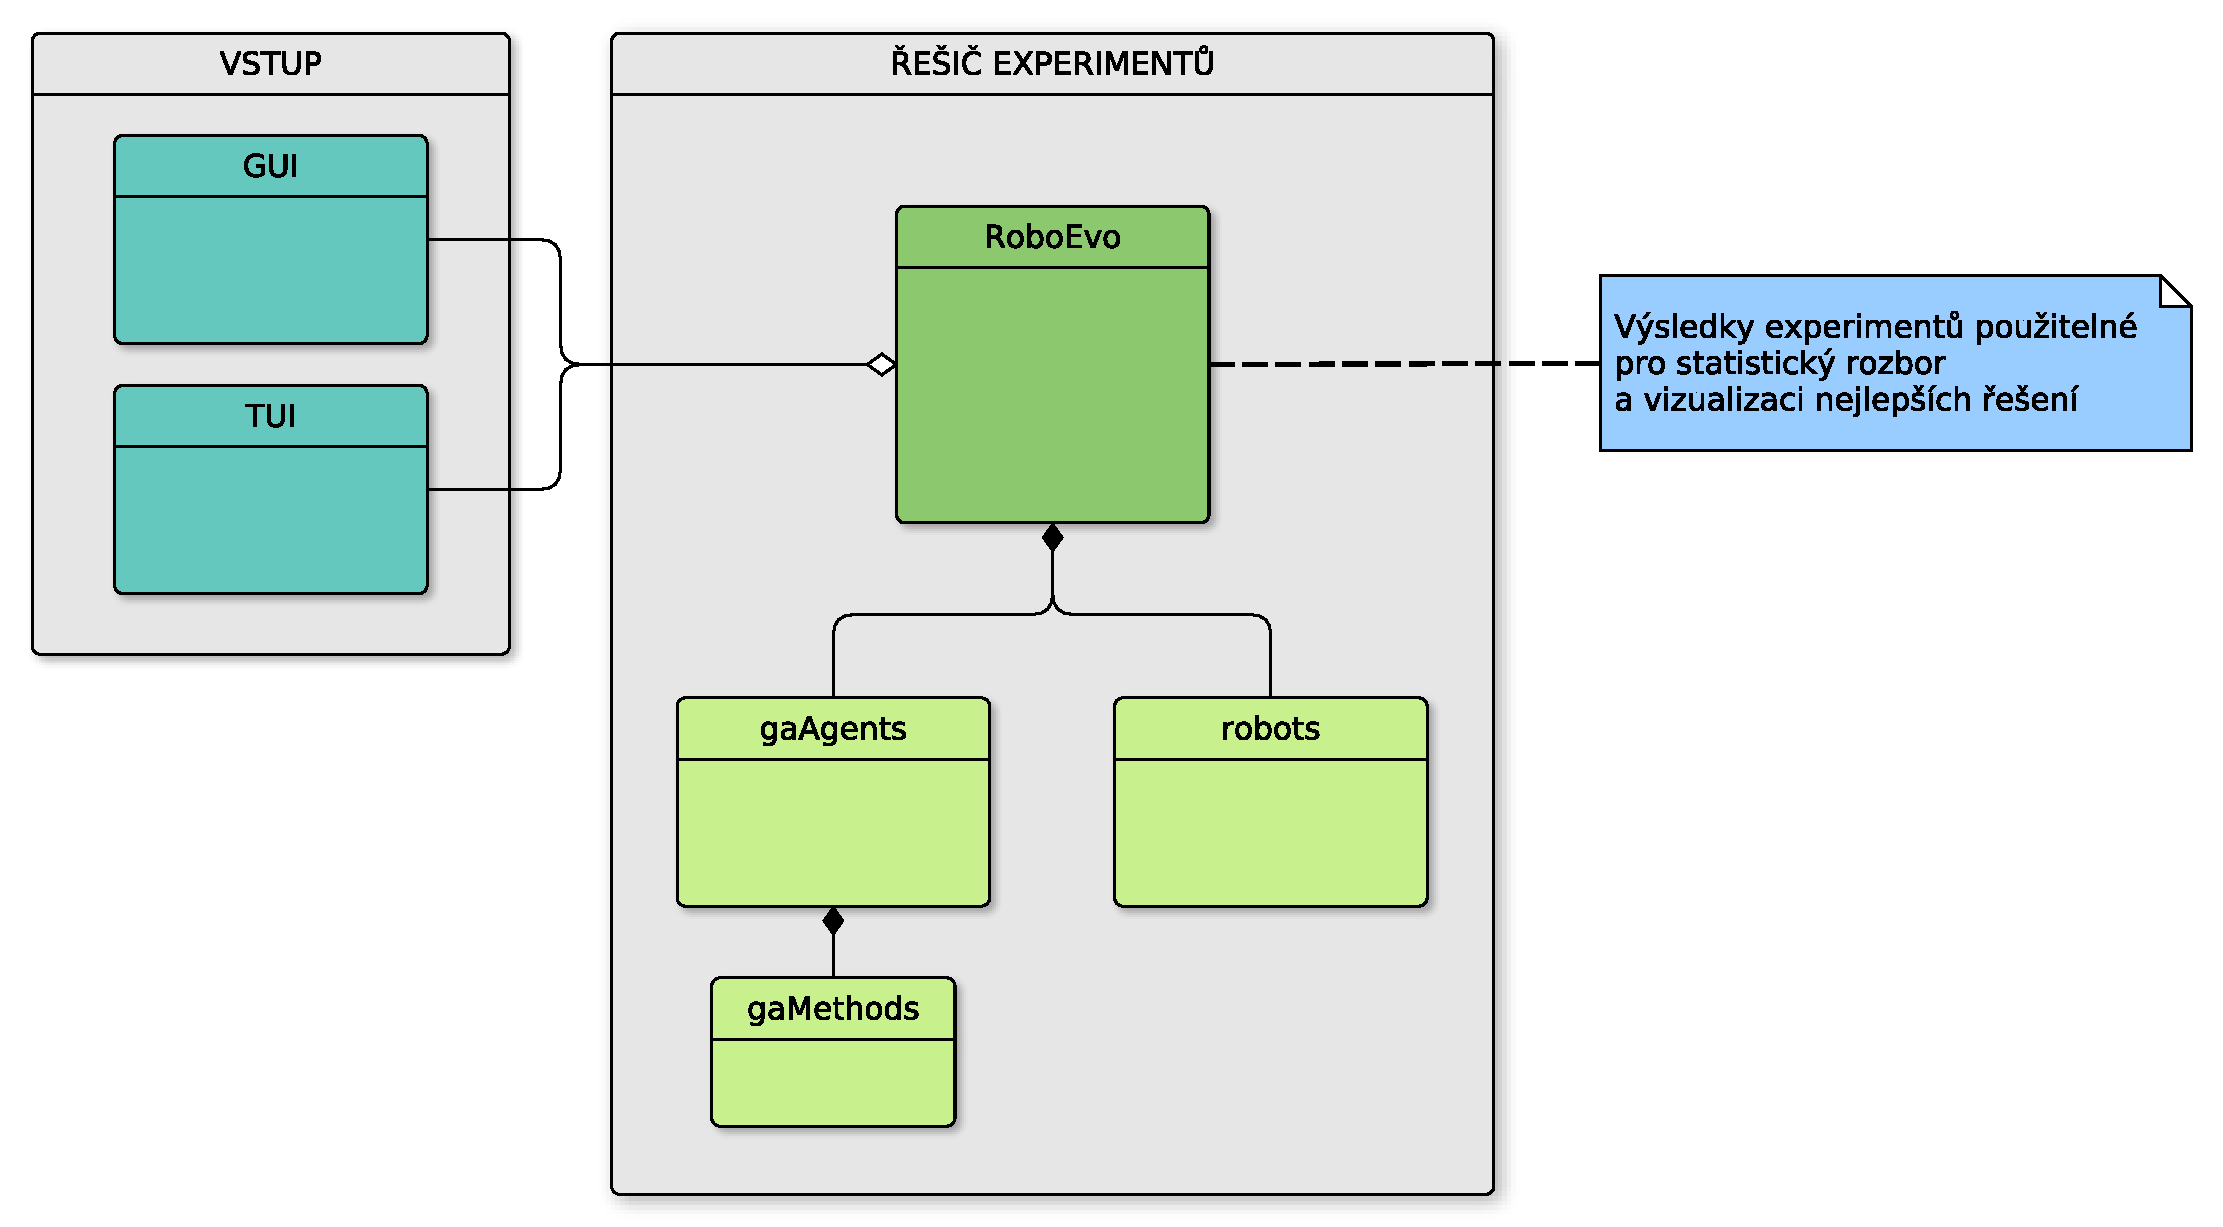
\includegraphics[width=1\textwidth]{../img/BP_imp_graph.pdf}
    \caption{Struktura projektu}
    \label{fig:struktura}
\end{figure}

Obrázek \ref{fig:struktura} popisuje na jaké části je projekt rozdělen.
Centrální částí je modul \emph{RoboEvo}, pomocí kterého knihovna provádí
evoluční experimenty. Tento modul se pro přehlednost a rozšířitelnost kódu
skládá z několika menších částí -- \emph{gaAgents} (popisující agenty a vlastní
genetické operátory) a \emph{robots} (udržující jednotný způsob přístupu k
různým robotům). 

Jak popisují funkční požadavky (v sekci \ref{Specifikace-funkčnípožadavky}),
projekt umožňuje několik možných způsobů práce s naší knihovny. Dva základní
možné přístupy jsou za pomoci grafického, nebo textového rozhraní. Tyto
přístupy jsou v projektu rozděleny do \emph{GUI} (\emph{Graphical User
Interface}) a \emph{TUI} (\emph{Text-based User Interface}) modulů. Uživatel,
který bude chtít pracovat s kódem části knihovny zaměřené na vytváření a
provádění experimentů s evolučním vývojem, se dále může zaměřit na hlavní modul
\emph{RoboEvo} (a s ním spojené pomocné moduly).

\paragraph{} 
Dále v této kapitole v sekci \ref{imp:roboevo} popíšeme centrální modul
\emph{RoboEvo} pracující s několika dalšími pomocnými moduly, jejichž
implementace popíšeme v dalších oddílech. Popíšeme třídu agentů v oddílu
\ref{imp:gaAgents}. Implementace vlastních genetických operátorů se nachází v
oddílu \ref{imp:gaMethods}. Vlastní třída \emph{robots} propojující roboty ze
simulátoru \emph{MuJoCo} (MuJoCo popsáno v základních pojmech v oddílu
\ref{MuJoCo}) s ostatními třídami je vysvětlena (v oddílu \ref{imp:robots}).
Následně si moduly umožňující uživateli práci s knihovnou buď pomocí grafického
prostředí (v sekci \ref{imp:GUI}), nebo pomocí příkazové řádky (v sekci
\ref{imp:TUI}). Jako poslední (v sekci \ref{imp:experimentsetter}) si
představíme implementaci třídy \emph{experimentSetter}, sloužící k uchování a
předvolbě parametrů pro experimenty a usnadňující tak provádění většího
množství experimentů.

\section{RoboEvo a pomocné moduly}
V této sekci popíšeme hlavní modul \emph{RoboEvo} a jeho pomocné moduly\\
\emph{gaAgents}, \emph{gaMethods} a \emph{robots}. Soubor těchto modulů tvoří
hlavní část celého projektu, obsahující celý proces umožňující provádění
evolučních experimentů s roboty. Vybrané rozdělení modulů bylo vytvořeno pro
zjednodušení čitelnosti a rozšířitelnosti kódu, kde nyní každý modul
zprostředkovává velmi specifickou roli v procesu evolučního vývoje, a tudíž je
pro uživatele jednoduché tyto části upravovat. Tato část projektu je zároveň
zcela oddělena od zpracování uživatelského vstupu, který do hlavního modulu
vstupuje z vnějších modulů, až ve chvíli zahájení experimentu. 

\subsection{Modul RoboEvo} \label{imp:roboevo}
Modul \emph{RoboEvo} je centrální modul tohoto projektu, sloužící pro spouštění
a běh experimentů s evolučním vývojem robotů. 

Každý experiment se skládá z několika nezávislých částí. Experiment může
využívat různé typy evolučních agentů s různými genetickými operátory a může se
snažit vyvíjet různé typy robotů. Jak bylo zmíněno výše, tyto částí jsou pro
přehlednost, čitelnost a rozšířitelnost kódu oddělené do vlastních menších
implementací, rozšiřující hlavní modul (jednotlivé implementace budou popsány v
dalších oddílech). 

\paragraph{Implementace modulu \emph{RoboEvo}}
Tento modul obsahuje funkce sloužící jak k inicializaci evolučních experimentů,
tak k samotnému běhu evolučních algoritmů, včetně propojení s knihovnou
\emph{Gymnasium} od Farama Foundation (popsáno v sekci \ref{Simulátory -
Porovnání}), zprostředkovávající simulaci fyzikálního prostředí pro testování
jedinců.

Hlavní funkcí, která z vnějšího vstupního prostředí (např. \emph{GUI},
\emph{TUI}, vlastní modul uživatele) přijímá parametry pro spuštění
experimentů, je funkce \linebreak\texttt{run\_experiment}. Povinným parametrem
této funkce jsou parametry \linebreak experimentu, které jsou pro zapouzdření
vloženy do jednoduché třídy \linebreak\texttt{ExperimentParams} (modul
\emph{experiment\_params}) obsahující následující hodnoty:

%TODO: LOOK AT BLACK BARS FOR LINEBREAKS \linebreak

%TODO: care for params changes - show graph (possibly)
\begin{itemize}
    \item \texttt{robot} -- zvolený robot z modulu \texttt{robots},
    \item \texttt{agent} -- zvolený agenta z modulu \texttt{gaAgents},
    \item \texttt{ga\_population\_size} -- velikost populace jedinců v
        evolučním algoritmu,
    \item \texttt{ga\_generation\_count} -- počet generací, po které bude
        evoluční algoritmus běžet,
    \item \texttt{show\_best} -- příznak určující, zda po doběhnutí evolučního
        algoritmu \\chceme v simulovaném prostředí zobrazit řešení nejlepšího
        jedince,
    \item \texttt{save\_best} -- příznak určující, zda po doběhnutí evolučního
        algoritmu \\chceme uložit nejlepšího jedince,
    \item \texttt{save\_dir} -- cesta ke složce, kam chceme uložit data z běhu
        evolučního algoritmu (pokud neexistuje, je složka automaticky vytvořena
        po doběhnutí algoritmu),
    \item \texttt{note} -- případná poznámka, kterou může uživatel speciálně
        odlišit název dat, ukládaných po doběhnutí algoritmu.
\end{itemize}

Funkce \texttt{run\_experiment} zpracovává tyto parametry a zajišťuje vše
potřebné pro běh experimentu. V přípravě probíhá spouštění výpočetních
jednotek pro paralelizaci testovacího prostředí (umožňující ohodnocení
populace jedinců paralelně). Následně proběhne spuštění evolučního algoritmu se
zvolenými parametry, po kterém funkce uloží data vygenerovaná evolučním
algoritmem -- fitness hodnoty jedinců v každé generaci, celá
populace jedinců z poslední generace a (volitelné) nejlepší řešení na konci
experimentu. Tato data jsou uložená do složky, dostupné na cestě popsané v
\texttt{save\_dir} parametru.

% \pagebreak
% Těmito parametry jsou:
% \begin{itemize}
    % \item \texttt{-{}-experiment} -- argument přijímající textový vstup
    %     specifikující jméno experimentu, jehož parametry chceme načíst a
    %     spustit (pracující s modulem \texttt{experiment\_setter} popsaného v
    %     oddíle \ref{imp:experimentsetter}),
    % \item \texttt{-{}-experiment\_names} -- při výběru tohoto argumentu při
    %     spuštění programu program vypíše názvy všech dostupných vytvořených
    %     experimentů z modulu \texttt{experiment\_setter} a následně se ukončí,
    % \item \texttt{-{}-batch} -- argument přijímající číselnou hodnotu,
    %     specifikující kolikrát se má nakonfigurovaný experiment opakovaně
    %     spustit (používané pro statistické vyhodnocení výsledků experimentů),
    % \item \texttt{-{}-batch\_note} -- textový argument umožňující připojit
    %     vlastní poznámku k názvu složky, do které se experimenty z
    %     několikanásobného spuštění ukládají (argument nemá žádný efekt pro
    %     experimenty z modulu \texttt{experiment\_setter}),
    % \item \texttt{-{}-open} -- textový argument přijímající cestu k uloženým
    %     datům nejlepšího jedince z libovolného předchozího experimentu,
    %     umožňující vizualizaci řešení daného jedince.
% \end{itemize}

\paragraph{Běh evolučního algoritmu}
Funkce \texttt{run\_experiment} zajišťuje spuštění evolučního algoritmu se
zvolenými parametry. Samotný běh evolučního algoritmu je poté zajištěn funkcí
\texttt{run\_evolution}. V rámci této funkce provádíme všechny kroky evolučního
algoritmu (jak byly popsány v základních pojmech evolučních algoritmů v sekci
\ref{Evoluční algoritmy}). Navíc zde pro jedince vytváříme simulační prostředí,
ve kterých budou jedinci testováni při výpočtu fitness.

Po výpočtu fitness přichází na řadu genetické operátory, které jsou vždy
specifické pro zvolený evoluční algoritmus. V naší implementaci jsou zvolené
operátory specifikované v třídě agenta. Podrobněji třídu agentů
popíšeme v dalším oddíle \ref{imp:gaAgents}.
%TODO: zmínit genotype phenotype mapping v základních pojmech

V rámci této funkce se zároveň sbírají důležitá data o vývoji fitness hodnot
napříč všemi generacemi a pokud to uživatel povolil, jsou aktuální data v
průběhu algoritmu vykreslována do jednoduchého grafu.

\subsection{Modul \emph{gaAgents}} \label{imp:gaAgents}
Modul \emph{gaAgents} je kolekcí několika tříd popisující agenty využívané
evolučními algoritmy. Každá třída agenta povinně obsahuje několik funkcí, které
specifikují jak vypadá genotyp jedinců vytvořených podle tohoto agenta, jakým
způsobem se generuje populace takových jedinců, jaké genetické operátory budou
při evolučním vývoji použité a jakým stylem probíhá transformace genotypu
jedince na nastavení odpovídajících aktuátorů robota (tzv.
\emph{genotype-phenotype mapping}). 

\paragraph{Třída agenta}
Hlavní třídou tohoto modulu, tvořící šablonu pro všechny další definované
agenty, je třída \texttt{BaseAgent}. Všechny třídy popisující agenty mají
povinnost odvozovat od této třídy základního agenta. Součástí této třídy je
několik abstraktních metod (metody, které odvozená třída má povinnost
implementovat, aby byla použitelná). Výčet abstraktních metod agenta:

\begin{enumerate}[a)]
    \item metody využívané evolučním algoritmem:
        \begin{itemize}
            \item \texttt{generate\_population(population\_size)} -- metoda
                vytvářející populaci jedinců požadované velikosti,
            \item \texttt{get\_action(individual, step)} -- metoda
                zprostředkovávající transformaci genotypu jedince (popsaného v
                parametru \texttt{individual}) na fenotyp (vektor hodnot
                popisující nastavení aktuátorů pro ovládaného robota) v daném
                okamžiku (popsaným parametrem \texttt{step}),
            \item \texttt{selection(population, fitness\_values)} -- genetický
                operátor -- metoda přijímající populaci jedinců a jejich
                fitness hodnoty, vracející nějakým způsobem vybrané jedince,
            \item \texttt{crossover(population)} -- genetický operátor --
                metoda přijímající populaci jedinců (skupina rodičů ze
                selekce), na které provede křížení genotypů a vrátí vytvořenou
                skupinu potomků,
            \item \texttt{mutation(population)} -- genetický operátor -- metoda
                přijímající skupinu potomků, na kterých provede mutaci jejich
                genotypu a vrátí zmutované potomky,
        \end{itemize}
    \item metody využívané pro vstupní rozhraní:
        \begin{itemize}
            \item \texttt{for\_GUI(cls)} -- metoda vytvářející agenta s
                výchozím nastavením, který je využíván při prezentaci agenta v
                \emph{GUI},
            \item \texttt{description(self)} -- metoda, do které můžeme vložit
                text, sloužící jako rozsáhlejší popisek agenta v \emph{GUI}.
        \end{itemize}
\end{enumerate}

Využití abstraktních metod se pro tuto implementaci hodí, protože tímto
způsobem můžeme v experimentech jednoduše zaměňovat typy využívaných
agentů a měnit tak průběh evolučního vývoje. 

\paragraph{Vlastní agent}
Uživatel pak může jednoduše přidávat vlastní agenty, vytvořením třídy odvozené
od třídy \texttt{BaseAgent} a implementováním potřebných metod. Pro
zjednodušení tohoto procesu, uživatel nemusí vlastnoručně programovat všechny
tyto metody, ale může využít připravené genetické operátory, implementované v
pomocném modulu \emph{gaMethods}, který si představíme v následujícím oddílu
\ref{imp:gaMethods}. Pokud uživatel nenajde takovou funkci, která by přesně
odpovídala jeho požadavkům, může si potřebný algoritmus dopsat sám, za dodržení
pravidel specifikovaných implementací třídy agenta.

\paragraph{Existující agenti}
V následujícím seznamu krátce představíme všechny dostupné agenty připravené
pro experimenty:

\begin{itemize}
    \item \textbf{\emph{StepCycleHalfAgent}} -- agent, jehož genotyp je vektor předem
        zvolené délky pro polovinu aktuátorů robota, kde hodnoty v genotypu přímo
        popisují nastavení aktuátorů. Tato nastavení jsou periodicky opakována
        v periodě zvolené délky. Nastavení aktuátorů je přeneseno na druhou
        polovinu aktuátorů s opačným znamínkem.
    \item \textbf{\emph{SineFuncFullAgent}} -- agent, jehož genotyp popisuje nastavení
        sinus funkce pro každý aktuátor robota (amplituda, frekvence, posun v
        ose $x$ a posun v ose $y$). Nastavení aktuátoru je pak vygenerované
        výpočtem sinus funkcí v daném časovém okamžiku (z parametru
        \texttt{step} funkce \texttt{get\_action}).
    \item \textbf{\emph{SineFuncHalfAgent}} -- agent, stejný jako
        \emph{SineFuncFullAgent}, který ale má nastavení sinus funkcí pouze pro
        polovinu aktuátorů robota. Druhou polovinu generuje převrácením hodnot
        z první polovinu.
    \item \textbf{\emph{FullRandomAgent}} -- agent, podobný agentovi
        \emph{StepCycleHalfAgent}, generující do svého genotypu nastavení pro všechny
        aktuátory robota. Tato nastavení se opět periodicky opakují se zvolenou
        velikostí periody.
    \item \textbf{\emph{TFSAgent}} -- složitější agent než \emph{SineFuncFullAgent},
        využívající genotyp popisující zkrácenou Fourierovu transformaci pro
        každý aktuátor na generování požadovaného nastavení. Genotyp obsahuje
        parametry pro amplitudy a posuny pro vybraný počet sinus funkcí.
        Výpočet nastavení jednoho aktuátoru potom vypadá dle následující
        rovnice:

        \begin{equation}
            \text{nastavení aktuátoru} = \sum_{i=1}^{N}A_i\cdot\sin\frac{i\cdot
            step\cdot2\pi}{T} + \delta_i
        \end{equation}

        kde $N$ je pevný počet součtů, na které se omezíme, $T$ je pevně
        zvolená perioda, $A_1,...,A_N$ je $N$ amplitud pro sčítané sinusoidy a
        $\delta_i,...,\delta_N$ je $N$ posunů.
\end{itemize}

\subsection{Modul gaMethods} \label{imp:gaMethods}
%TODO gaMethods

\subsection{Roboti} \label{imp:robots}
%TODO robots

\section{Grafické rozhraní} \label{imp:GUI}
%TODO GUI

\section{Textové rozhraní} \label{imp:TUI}
%TODO TUI

\section{Třída experimentů} \label{imp:experimentsetter}
%TODO experiment_setter


\chapter{Experimenty a výsledky} \label{chapter-experimenty}

V této kapitole se podíváme na tři typy experimentů, které s naším systémem
můžeme provádět. Knihovna implementuje několik různých přístupů, jak roboty
řídit a jak je vyvíjet pomocí evolučních algoritmů. Následující experimenty
předvedou vzorek z těchto přístupů. 

Cílem všech následujících experimentů je pomocí evolučních algoritmů vyvinout
zvoleného robota tak, aby byl schopný stabilního pohybu v simulovaném prostředí
v předem určeném směru. Každý jedinec začíná svůj simulační běh v~prostředí v
počátku na souřadnicích $(0,0)$. V našem experimentu chceme, aby~se robot
pohyboval ve směru rostoucí x-ové souřadnice. Kvalita jedinců je pak jednoduše
vypočtena dle následující rovnice:

\begin{equation} \label{fitness_calc}
    fitness = x - 0.5\cdot|y|
\end{equation}
kde $(x,y)$ jsou souřadnice bodu v simulovaném prostředí, do kterého jedinec
dorazil (buď do vypršení limitovaného času na simulaci, nebo do dosažení
podmínky předčasně ukončující simulační běh -- např. pádu robota).

V prvním experimentu v sekci \ref{exp1} si ověříme přirozený předpoklad, že pro
řízení jednoduchých robotů nám stačí základní evoluční algoritmy a pro
složitější roboty (s větším množstvím stupňů volnosti) potřebujeme pokročilé
přístupy. V~následujících dvou experimentech v sekci \ref{exp2} popíšeme
experimenty demonstrující možnost evolučního vývoje jak řízení, tak morfologie
robotů.

\section{Vývoj řízení robotů} \label{exp1}

V této sekci se zaměříme na vývoj řízení robotů. Řízení robota je systém,
který na základě vstupů z prostředí (senzory robota, čas atd.) generuje
signály do výkonných prvků robota (typicky motory). 

Průběh vývoje řízení robota je ovlivněn zvoleným agentem, který definuje
genotyp jedinců a určuje, jaké genetické operátory budou při vývoji využívány.
Podrobnější popis agentů se nachází v sekci \ref{imp:gaAgents}.

První pokus se bude snažit vyvinout řízení pro pokročilého robota v projektu
označovaném jako \emph{SpotLike} (na obrázku \ref{imp:fig:robots.SpotLike}, blíže
popsaný v implementaci v~sekci \ref{imp:robots.Spot}). Jedná se o robota
kráčejícího na čtyřech nohách, kde každá noha má 3~stupně volnosti (tedy celkem
12 pro celého robota). Můžeme ho tedy řadit mezi roboty, u kterých již bude
obtížnější vyvinout stabilní pohyb v určeném směru.

Kráčení, kterého bychom u robotů chtěli dosáhnout, si můžeme představit jako
periodický pohyb, kde každá noha cyklicky opakuje stejné pohyby. Proto se pro
vývoj řízení pokusíme využít agenty, kteří interně podle parametrů generují
periodické hodnoty pro motory robotů. 

\paragraph{Volba parametrů velikosti experimentu}
Pro tento typ experimentu inicializujeme populaci se \textbf{100 jedinci}.
Abychom zjistili, kolik generací je potřeba pro rozumné výsledky, necháme
nejprve proběhnout delší experiment, ve kterém vývoj evolučního algoritmu
poběží po \textbf{500 generací}. Abychom vyloučili vliv náhodné inicializace
populace jedinců v genetickém algoritmu, pro vyhodnocení je celý
běh algoritmu \textbf{20krát} nezávisle opakován a výsledky prezentujeme
pomocí následujícího typu grafu.

\begin{figure}[!htb]
    \centering
    \includegraphics[width=1\textwidth]{../img/BIGexperiment1_TFS_10ticks.pdf}
    \caption{Velký experiment, 20 opakování algoritmu po 500 generacích, robot
    \emph{SpotLike}, agent \emph{TFSAgent}}
    \label{fig:exp_big}
\end{figure}

\paragraph{Krabicový graf}
Pro vizualizaci dat využíváme krabicový graf (boxplot). Tento graf vizualizuje
statistické rozložení dat pomocí kvartilů. Uprostřed se nachází \emph{krabice}
(obdélník), který je shora ohraničena 3. kvartilem a zespodu 1. kvartilem.
Rozsah pokrytý obdélníkem tedy obsahuje 50 \% pozorovaných hodnot. Uvnitř
\emph{krabice} se nachází (v našich grafech oranžovou barvou) čára, naznačující
hodnotu mediánu. Dále krabicové grafy nad a pod střední \emph{krabicí}
vykreslují tzv. \emph{vousy}, což vizualizuje variabilitu dat nad 3. a pod 1.
kvartilem. Vousy nad a pod krabicí mají stejnou délku rovnající se 1.5 násobku
rozdílu mezi 3. a 1. kvartilem. Dále se v grafu mohou nacházet odlehlé body
(\emph{outliers}). To jsou hodnoty mimo krabici a vousy. Odlehlé body které
jsou vykresleny jako samostatné kroužky.

Grafy vznikají složením dat z průběhů fitness hodnot několika opakování daného
evolučního algoritmu. Jeden krabicový diagram pro danou generaci zobrazuje
rozložení hodnot fitness všech jedinců dané generace ze všech běhů. V grafu
\ref{fig:exp_big} je to celkem 2000 hodnot. V poslední generaci dále červené
značky označují hodnotu maximální fitness v jednotlivých bězích. 

V našich grafech pro přehlednost dále vykreslujeme hodnotu maximální (modrou
čarou) a minimální (červenou čarou) fitness v dané generaci.

Krabicový graf na obrázku \ref{fig:exp_big} zobrazuje vyhodnocení popsaného
velkého experimentu. Z grafu můžeme vidět, že největší růst fitness proběhl
přibližně v~prvních 200 generacích. Optimalizace dále pokračovala a byla
schopná nacházet řešení s lepším hodnocením, ale pro účely vyhodnocování našich 
experimentů bude dostačující, když evoluci v tomto experimentu omezíme na 200
generací a algoritmus necháme vývoj pětkrát nezávisle zopakovat. To se nám
ukázalo jako dostatečné množství dat, které se podobá předvedenému velkému
experimentu a~můžeme tak urychlit statistické vyhodnocení. 

Průběh předvedeného experimentu v obrázku \ref{fig:exp_big} trval přibližně 12
hodin i~s~využitím paralelizace ohodnocení jedinců mezi 12 vláken na výkonném
osobním počítači. Díky omezení dalších experimentů na menší počet generací a
opakování algoritmu jsme schopni na stejném systému následující experimenty
provést v~řádech desítek minut.

\paragraph{První experiment}
Nejprve se pokusíme řízení robota \emph{SpotLike} (popsán v sekci
\ref{imp:robots.Spot}) vyvinout pomocí evolučního algoritmu, který kóduje
nastavení aktuátorů pomocí základních periodických funkcí (agent
\emph{SineFuncFullAgent} popisující tento algoritmus je popsán v implementaci v
sekci \ref{imp:gaAgents.sinefuncfullagent}). Každý aktuátor robota má v~tomto
případě přiřazenou vlastní periodickou funkci a genotyp jedinců specifikuje
parametry těchto periodických funkcí (4 parametry pro každý kloub -- amplituda,
frekvence, $x$ a $y$ posun). Funkce jsou popsány rovnicí (\ref{sinefunc}) v
sekci implementace agentů.

Evoluční algoritmus běžel \textbf{200 generací} se \textbf{100} náhodně
inicializovanými jedinci. Pro vyhodnocení byl celý běh evolučního algoritmu
pětkrát opakován vždy s novou náhodně vygenerovanou počáteční populací.

\begin{figure}[!h]
    \centering
    \includegraphics[width=1\textwidth]{../img/experiment1_Sine_10ticks.pdf}
    \caption{Vývoj fitness populace v experimentu se základním agentem\\
    \emph{SineFuncFullAgent} a robotem \emph{SpotLike}}
    \label{exp:first_sinefull}
\end{figure}

Graf na obrázku \ref{exp:first_sinefull} zobrazuje vývoj fitness
hodnot za běhu výše popsaného evolučního algoritmu. Data jsou vytvořena
kombinací záznamů o fitness hodnotách v dané generaci ze všech pěti nezávislých
běhů.

Graf ukazuje, že tento přístup vývoje řízení dosáhl maximální hodnotu fitness
okolo 15 a populace na této hodnotě stagnovala a nebyla schopna většího posunu.

\paragraph{Pokročilý agent}
Pro porovnání jsme zvolili pokročilého agenta \emph{TFSAgent}, který generuje
signály do aktuátorů pomocí omezených Fourierových řad (agent byl popsán v
sekci \ref{imp:gaAgents.TFSagent}). Tento agent je na úkor malého zvětšení
genotypu, oproti předchozímu agentovi schopný generovat mnohem komplexnější
periodické funkce popsané skládáním několika funkcí sinus. V našem příkladě
byly na nastavení složeny $3$ sinusové funkce.

Stejně jako v předchozím běhu, algoritmus běžel 200 generací se 100 jedinci
a~byl opět pětkrát zopakován.

\begin{figure}[!h]
    \centering
    \includegraphics[width=1\textwidth]{../img/experiment1_TFS_10ticks.pdf}
    \caption{Vývoj fitness populace v experimentu s pokročilým agentem
    \emph{TFSAgent} a se stejným robotem \emph{SpotLike}}
    \label{exp:first_TFS}
\end{figure}

Graf \ref{exp:first_TFS} vývoje fitness hodnot z experimentu s pokročilým
agentem ukazuje, že tento agent již byl schopný vyvinout stabilní pohyb i pro
zadaného komplexního robota. Maximální fitness hodnota, které při vývoji agent
dosáhl, se pohybovala okolo 60. Zároveň podle krabicového grafu vidíme, že
poměrně velká část populace byla schopná dosáhnout výsledků, přesahující
nejlepší výsledky jednoduššího agenta.

\paragraph{}
Z experimentů jsme zároveň dostali i nejlepšího jedince z poslední generace
evolučního algoritmu. Jelikož naše simulované fyzikální prostředí je
deterministické, můžeme řešení nejlepšího jedince zpětně vizualizovat.

Ruční kontrolou těchto výsledků jsme dále zjistili, že pouze část (dva z pěti
běhů) dosáhly takového pohybu, který bychom od robota této morfologie
očekávali. Tělo v robota v těchto případech (až na menší odchylky) směřovalo
rovně, způsobem připomínající chůzi čtyřnohých zvířat podobné morfologie. Zbylé
běhy vyvinuly stabilní, ale ne zcela estetickou chůzi. Roboti se v těchto
případech posouvali stranou využitím většího rozsahu v rotaci
(\emph{kyčelních}) kloubů. Pravděpodobně kvůli lepší stabilitě robota.

Osobně si myslím, že vývoj estetického pohybu pro tohoto robota je s malou
úpravou hodnotící funkce možný. Ta by například mohla penalizovat rotaci těla
od požadovaného směru pohybu. Chůze stranou je kvůli rozsahu (\emph{kyčelních})
kloubů (hlavně v ose délky těla robota) mnohem snazší na vyvinutí, a tak tento
způsob chůze tvoří silné lokální optimum. Agenti velmi rychle konvergují ke
způsobům chůze, které jsou stabilní, což jim navyšuje šanci urazit větší
vzdálenost bez pádu. Chůze stranou je oproti vratké chůzi rovně mnohem
stabilnější. Navržená jednoduchá úprava hodnotící funkce by měla být schopna
toto lokální optimum penalizovat, a tedy vynutit estetičtější pohyb.

\paragraph{}
Ve srovnání s předchozími pokusy jsme se pomocí stejných agentů snažili
vyvinout řízení jednoduššího robota označeného jako \emph{AntV3} (zobrazeného na
obrázku \ref{imp:fig:robots.AntV3}, blíže popsán v implementaci v sekci
\ref{imp:robots.Ant}). Můžeme ho brát jako jednoduššího, protože obsahuje menší
počet kloubů (8 stupňů volnosti) v porovnání s~robotem \emph{SpotLike}. Zároveň
jeho morfologie umožňuje snazší pohyb všemi směry s menším rizikem pádu.

Řízení jsme vyvíjeli pomocí agentů se stejnými parametry jako v případě s
pokročilým robotem. Celý běh byl opět pro statistické vyhodnocení pětkrát
opakován se stejnou velikostí náhodně vygenerované populace (\textbf{100
jedinců}). Jelikož jsme kvůli menšímu počtu stupňů volnosti očekávali schopnost
agentů vyvinout řízení rychleji, zkrátili jsme délku evoluce na \textbf{100
generací}.

\begin{figure}[h!]
    \centering
    \includegraphics[width=1\textwidth]{../img/experiment1_2_Sine_10ticks.pdf}
    \caption{Vývoj fitness populace se základním agentem
    \emph{SineFuncHalfAgent} a~jednodušším robotem \emph{AntV3}}
    \label{exp:first2_sinefull}
\end{figure}
\begin{figure}[h!]
    \includegraphics[width=1\textwidth]{../img/experiment1_2_TFS_10ticks.pdf}
    \caption{Vývoj fitness populace s pokročilým agentem \emph{TFSAgent} a
    jednodušším robotem \emph{AntV3}}
    \label{exp:first2_TFS}
\end{figure}

Z vývoje fitness (v grafu \ref{exp:first2_sinefull} a \ref{exp:first2_TFS})
můžeme pozorovat, že oba agenti byli schopní u tohoto jednoduššího robota
dosáhnout přijatelných výsledků i s omezeným počtem generací. Přijatelné
výsledky jsou částečně podpořeny faktem, že~i~náhodné konfigurace mají dobrou
šanci tohoto robota rozpohybovat v požadovaném směru, a tedy již velmi brzy
získat dobré ohodnocení. To se zároveň projevuje i na minimální fitness. Pro
tohoto robota je totiž stejně jednoduché dostat takovou konfiguraci aktuátorů,
které ho rozpohybují v opačném směru (jedinec z definice hodnotící funkce
obdrží záporné ohodnocení).

\section{Vývoj řízení a morfologie robotů} \label{exp2}

V této sekci předvedeme dva další typy experimentů, které naše knihovna
podporuje -- simultánní vývoj (v sekci \ref{exp2:para_evo}) a oddělený
vývoj (v sekci \ref{exp2:split_evo}) řízení a morfologie.

Tyto experimenty se od předchozích liší tím, že evolučnímu algoritmu povolíme
vyvíjet i zvolené části těla robota. To teoreticky umožní z těla původního
robota vyvinout optimálnější morfologii pro zadaný problém.

Vývoj těla je implementací umožněn díky speciálním značkám v XML konfiguračních
souborech (popsaných v konfiguraci vlastního robota v sekci \ref{imp:robots}).

\subsection{Simultánní vývoj řízení a morfologie} \label{exp2:para_evo}

V prvním příkladu předvedeme experiment, ve kterém umožníme evolučnímu
algoritmu vyvíjet zároveň řízení i morfologii robota. Tento experiment by
teoreticky mohl pomáhat v optimalizaci morfologie robotů za hranici
představivosti jejich autorů. 

Pro vývoj morfologie volíme při inicializaci agenta \emph{masku} těla robota
(popsána v parametru \texttt{body\_part\_mask} v sekci \ref{imp:robots}). Tato
maska popisuje, které části těla mají při vývoji zůstat beze změny (hodnota
\texttt{False}) a zároveň určuje povolené rozsahy hodnot pro~části těla
otevřené pro evoluční vývoj.

Kvalita jedinců byla v tomto experimentu hodnocena stejně jako v předchozích
experimentech. Cílem pro jedince je tedy dojít co nejdále v určeném směru.
Přesný výpočet fitness je popsán rovnicí (\ref{fitness_calc}). 

Pro experiment jsme zvolili robota \emph{AntV3} (popsán v implementaci v sekci
\ref{imp:robots.Ant}). Tento typ experimentů je ale samozřejmě povolen pro
libovolného robota, který umožňuje evoluční vývoj alespoň jedné části těla.

\paragraph{Vývoj robota \emph{AntV3}}
Jak bylo řečeno v této ukázce jsme zvolili robota \emph{AntV3}. Pro vývoj
robota byl využit agent \emph{SineFuncHalfAgent} (popsaný v sekci
\ref{imp:gaAgents.sinefunchalfagent}). \emph{AntV3} je robot se složitější
morfologií končetin a z tohoto důvodu ho vybíráme pro demonstraci tohoto typu
vývoje.

Tento experiment je nakonfigurovaný v modulu \emph{experiment\_setter} pod
názvem \texttt{exp2\_body\_para}. Pro evoluční algoritmus byla zvětšena
velikost populace na \textbf{150 jedinců} (větší velikost populace je zvolena
kvůli rozšíření prohledávaného prostoru, ve kterém evoluce hledá optimální
řešení) a evoluci byl umožněn vývoj po \textbf{200 generací}. Zároveň byl
zvolen povolený rozsah délek částí končetin pro vývoj. Robot \emph{AntV3} (na
obrázku \ref{imp:fig:robots.AntV3}, popsaný v sekci \ref{imp:robots.Ant}) má 4
končetiny složené ze dvou částí -- pro jednoduchost je označme jako
\emph{stehno} a \emph{lýtko}. V~základní konfiguraci je délka \emph{stehna} pro
tohoto robota $0.2$ (pro vývoj byl zvolen rozsah mezi $0.1$ a $0.5$) a délka
\emph{lýtka} je $0.4$ (pro vývoj umožníme rozsah mezi $0.15$ a $0.5$). Délka
libovolné části těla je při vývoji nezávislá na ostatních.

\begin{figure}[h!]
    \includegraphics[width=1\textwidth]{../img/experiment2_para_10ticks.pdf}
    \caption{Vývoj fitness populace při současném vývoji řízení a morfologie
    s~agentem \emph{SineFuncHalfAgent} a robotem \emph{AntV3}}
    \label{exp:exp2_para}
\end{figure}

Z grafu na obrázku \ref{exp:exp2_para} můžeme pozorovat, že tento typ vývoje
zvládl stabilně produkovat vyšší fitness hodnoty než srovnatelný předchozí
experiment (využívající stejného agenta i robota) nevyužívající vývoje
morfologie (graf na obrázku \ref{exp:first2_TFS}). Můžeme tedy odhadovat, že
mohou existovat optimálnější konfigurace končetin tohoto robota, než ta
výchozí.

\begin{figure}[h!]
    \centering
    \begin{minipage}{0.5\textwidth}
        \centering
        \includegraphics[width=0.75\textwidth]{../img/crop_exp2_para_side1.jpg}
    \end{minipage}%
    \begin{minipage}{0.5\textwidth}
        \centering
        \includegraphics[width=0.75\textwidth]{../img/crop_exp2_para_top1.jpg}
    \end{minipage}
    \caption{Příklad z výsledků současného vývoje řízení a morfologie robota
    \emph{AntV3}}
    \label{fig:exp2_para_body_show}
\end{figure}

Díky možnosti přehrávání nejlepších řešení jednotlivých běhů algoritmu můžeme
zároveň prozkoumat, k jakým konfiguracím vývoj dospěl. Ukázalo se, že~vývoj
dospěl buď k robotům s velmi dlouhými končetinami, nebo (jak je na obrázcích
\ref{fig:exp2_para_body_show}) k robotům s několika dlouhými
(\emph{odrazovými}) končetinami a jednou kratší končetinou (sloužící jako
\emph{kormidlo}). 

Obrázky \ref{fig:exp2_para_body_show} ukazují nejúspěšnějšího robota z
předvedeného experimentu, který je schopný své tělo díky kratší zadní noze
naklonit, a je tak schopný poměrně rychle skákat vpřed.

\subsection{Oddělený vývoj řízení a morfologie} \label{exp2:split_evo}
V tomto experimentu předvedeme druhý typ vývoje řízení a morfologie robota, a
to oddělený vývoj. V tomto typu evolučního vývoje se nejprve provede vývoj
řízení robota s výchozí morfologií. Následně se vývoj řízení zafixuje ve stavu
populace z poslední generace a začne druhá část vývoje, ve kterém se vyvíjí
pouze morfologie robota.

Jedinci tak dostanou možnost nejprve vyvinout samotný pohyb (jak tomu bylo v
prvním experimentu) a následně evolučním vývojem optimalizovat tělo pro
specifický pohyb. Tímto přístupem by teoreticky jedinci měli být schopni
dosáhnout lepších výsledků než při vývoji samotného řízení.

Pro tento experiment jsme zvolili stejného robota (s totožnými rozsahy
velikostí končetin) a stejného agenta jako v předchozím experimentu.
Konfigurace experimentu je v modulu \emph{experiment\_setter} pod
názvem \texttt{exp2\_body\_serial}. Evoluční algoritmus běžel nejprve 100
generací, při kterých se vyvíjelo řízení robota a následně 100 generací pro
vývoj morfologie.

\begin{figure}[h!]
    \includegraphics[width=1\textwidth]{../img/experiment2_serial_10ticks.pdf}
    \caption{Vývoj fitness populace při odděleném vývoji řízení a morfologie
    s~agentem \emph{SineFuncHalfAgent} a robota \emph{AntV3}}
    \label{exp:exp2_serial}
\end{figure}

V grafu na obrázku \ref{exp:exp2_serial} můžeme pozorovat vývoj fitness v
jednotlivých generacích. Můžeme vidět, že po 100. generaci nastal malý pokles
průměrných hodnot fitness, což bylo zapříčiněno začátkem vývoje morfologie
robota. Ten začíná vygenerováním zcela náhodných konfigurací těla robota (v
povoleném rozsahu délek končetin), a tedy může chvilkově vést k horším
výsledkům. Časem ale vidíme, že evoluce byla schopná optimalizovat tělo robota
pro již vyvinutý pohyb, a tak celkově vylepšit výsledky jedinců.

\begin{figure}[h!]
    \centering
    \includegraphics[width=0.4\textwidth]{../img/crop_exp2_serial_top1.jpg}
    \caption{Příklad z výsledků odděleného vývoje řízení a morfologie robota
    \emph{AntV3}}
    \label{fig:exp2_serial_body_show}
\end{figure}

Na obrázku \ref{fig:exp2_serial_body_show} můžeme vidět nejlepšího jedince z
experimentu s odděleným vývojem řízení a morfologie. Jedná se zároveň o dobrý
příklad morfologie, ke které se řešení často blížila. Pro tento typ pohybu se 
robotům hodilo mít mnohem delší části končetin vedoucí přímo od těla
(\emph{stehno}), které svým pohybem jsou schopny posunout robota dále, a tak
optimalizovat uraženou vzdálenost.


\chapter*{Závěr}
Práce představuje platformu pro tvorbu a provádění experimentů s evolučními
algoritmy na simulovaných robotech. Práce splnila cíle, které pro ni byly
stanoveny. Vytvořili jsme systém přístupný uživatelům s různými úrovněmi
pochopení problematiky evolučních algoritmů a zpřístupnili tak nástroj, pomocí
kterého budou uživatelé moci jednoduše prohlubovat a aplikovat své znalosti.
Platforma nabízí řadu implementovaných operátorů evolučních algoritmů a několik
robotů různých úrovní složitosti, se kterými může uživatel okamžitě pracovat.

Při tvorbě platformy jsme dbali na to, aby zdrojový kód byl srozumitelný
a~jednotlivé části logicky rozdělené, což uživatelům umožní a zjednoduší
přístup ke zdrojovému kódu. Tím nabízíme možnost hlubšího pochopení fungování
evolučních algoritmů a jejich případného rozšiřování a aplikování nových
vlastních částí.

Experimenty provedené v této práci ukazují jak typy experimentů,
které~platforma umožňuje, tak styly jejich vyhodnocení. Pomocí experimentů jsme
na dvou robotech různých složitostí ověřili fakt, že jednoduché evoluční
algoritmy nestačí pro řešení všech problémů, a že pro určité pokročilé problémy
je třeba pokročilých evolučních algoritmů. 

Zároveň jsme demonstrovali příklady experimentů, které umožňují vývoj jak
řízení, tak morfologie robotů. Pro tento problém jsme v práci navrhli a
implementovali způsob, jakým je možné za běhu algoritmů měnit XML konfigurační
soubory robotů z knihovny \emph{MuJoCo}. Tyto experimenty předvedly zajímavé
výsledky, vytvářející roboty různých konfigurací, které byly schopné dosáhnout
lepších výsledků než ty výchozí.

Práce nabízí mnoho možností pro rozšiřování. Vedle pokročilejších evolučních
algoritmů na vývoj řízení robotů by zajímavým rozšířením mohlo být prozkoumání dalších
možností vývoje morfologie, umožňující rozsáhlejší změny v konfiguraci robotů.
Dalším by mohlo být podrobnější zkoumání dopadů různých fitness funkcí na
výsledky evolučního vývoje.

\addcontentsline{toc}{chapter}{Závěr}


%%% Seznam použité literatury
\include{literatura}

%%% Obrázky v bakalářské práci
%%% (pokud jich je malé množství, obvykle není třeba seznam uvádět)

% \listoffigures

%%% Tabulky v bakalářské práci (opět nemusí být nutné uvádět)
%%% U matematických prací může být lepší přemístit seznam tabulek na začátek práce.

% \listoftables

%%% Použité zkratky v bakalářské práci (opět nemusí být nutné uvádět)
%%% U matematických prací může být lepší přemístit seznam zkratek na začátek práce.
% \chapwithtoc{Seznam použitých zkratek}

%%% Přílohy k bakalářské práci, existují-li. Každá příloha musí být alespoň jednou
%%% odkazována z vlastního textu práce. Přílohy se číslují.
%%%
%%% Do tištěné verze se spíše hodí přílohy, které lze číst a prohlížet (dodatečné
%%% tabulky a grafy, různé textové doplňky, ukázky výstupů z počítačových programů,
%%% apod.). Do elektronické verze se hodí přílohy, které budou spíše používány
%%% v elektronické podobě než čteny (zdrojové kódy programů, datové soubory,
%%% interaktivní grafy apod.). Elektronické přílohy se nahrávají do SISu a lze
%%% je také do práce vložit na CD/DVD. Povolené formáty souborů specifikuje
%%% opatření rektora č. 72/2017.
\appendix
\chapter{Uživatelská dokumentace}
Platforma je uživateli přístupná pomocí dvou aplikací -- grafického a textového
rozhraní. Funkčnost aplikací byla otestována na operačních systémech Windows
a~Linux. Všechny aplikace jsou vytvořené v jazyce Python, a tedy všechny
soubory mají přípony \emph{.py}. 

Uživatelskou dokumentaci rozdělíme do dvou částí. V první v části
\ref{doc_1_spust_a_kompon} si popíšeme kroky potřebné ke spuštění aplikací a
předvedeme jednotlivá rozhraní a~práci s nimi. V druhé části
\ref{doc_2_experimenty} si poté předvedeme, jak se pomocí těchto rozhraní tvoří
a provádějí experimenty.

\section{Spuštění a komponenty rozhraní} \label{doc_1_spust_a_kompon}

V této sekci se nejprve podíváme, jak připravit prostředí se všemi potřebnými
knihovnami pro správné fungování celé platformy (v podsekci
\ref{doc_11_spust}). Dále si předvedeme uživatelská rozhraní -- grafické v
podsekci \ref{doc_12_GUI} a poté textové v~podsekci~\ref{doc_13_TUI}.

\subsection{Instalace a spuštění rozhraní} \label{doc_11_spust}
Celá platforma je vytvořená za pomoci několika knihoven, které musí být před
spuštěním nainstalované pro zajištění správné funkčnosti všech aplikací. Pro
usnadnění instalace všech potřebných knihoven bylo pomocí prostředí pro správu
balíčků \href{https://conda.org/}{\emph{Conda}} vytvořené vlastní prostředí, ve
kterém aplikace poběží. 

\paragraph{Instalace \emph{Conda}}

Uživatel nejprve musí nainstalovat \emph{Condu}. K tomu můžeme využít
minimalistický instalátor \emph{Miniconda} (dostupný na všech platformách
z~oficiálních stránek \url{https://docs.conda.io/en/latest/miniconda.html}).

Po stažení a instalaci tohoto instalátoru by měl uživatel mít z příkazové řádky
(popřípadě s využitím specializované \emph{Conda} příkazové řádky) přístup k
příkazu \texttt{conda}, který umožňuje ovládat prostředí pro správu balíčků. 

\paragraph{Tvorba prostředí}
Nyní můžeme v kořenové složce této práce využít následujícího příkazu pro
tvorbu prostředí pro naši aplikaci.
\begin{code}
conda env create -f conda_environment/environment.yml
\end{code}
Tento příkaz je volání aplikace \texttt{conda}. Pomocí spojení \texttt{env
create} specifikujeme, že chceme vytvářet nové prostředí pro běh aplikací.
Parameter \texttt{-f} příkazu říká, že bude následovat vstupní soubor (cesta ke
konfigurarčnímu souboru), pomocí kterého má být prostředí vytvořeno. Tento
konfigurační soubor se jménem \emph{environment.yml} je z pohledu kořenového
adresáře umístěn ve složce \emph{conda\_environment}.

Konfigurační soubor specifikuje detaily prostředí, jako jeho jméno (v našem
případě \emph{roboEvo}) a balíčky, které má nainstalovat.

Po doběhnutí instalace prostředí může být prostředí aktivováno pomocí příkazu
\texttt{conda activate roboEvo} a poté deaktivováno pomocí \texttt{conda
deactivate}. Pokud máme aktivované prostředí \emph{roboEvo}, všechny aplikace
naší platformy budou funkční.

\subsection{Grafické rozhraní -- \emph{GUI.py}} \label{doc_12_GUI}

S aktivovaným prostředím \emph{roboEvo} můžeme spustit grafické rozhraní.
Rozhraní je klasickou okenní aplikací, pomocí které může uživatel konfigurovat,
spouštět a zpětně vizualizovat experimenty s evolučním vývojem robotů.

Celé rozhraní je rozděleno do čtyř záložek, oddělující hlavní části potřebné
ke~tvorbě experimentů -- záložky \emph{Main}, \emph{Robot select}, \emph{Agent
config} a \emph{Evolution config}. Dále si zvlášť představíme jednotlivé
záložky.

\paragraph{Záložka \emph{Main}}
\begin{figure}[!htb]
    \centering
    \includegraphics[width=0.8\textwidth]{../img/GUI_main_tab.jpg}
    \caption{Úvodní okno aplikace}
    \label{doc_12_fig:GUI_main}
\end{figure}
Úvodní záložka grafické aplikace (obrázek \ref{doc_12_fig:GUI_main}), ve které
si můžeme prohlédnout zkrácený popis aktuálně nakonfigurovaného experimentu.
Tento popis je automaticky generován a aktualizován tak, aby reflektoval změny
konfigurace daného experimentu. 

Dále pod popisem experimentu najdeme tlačítka pro uložení aktuální konfigurace
a načtení dříve vytvořené konfigurace experimentu. Při ukládání experimentu
aplikace vytvoří okno s textovým polem pro pojmenování ukládané konfigurace. Po
zvolení jména je experiment uložen do souboru v pevně zvoleném adresáři. Při
načítání nějakého experimentu aplikace nabídne seznam všech dříve vytvořených
experimentů (jak vytvořených ve zdrojovém kódu, tak v okenní aplikaci), ze
kterého si uživatel může podle jména vybrat (aktuální konfigurace bude bez
možnosti obnovy přepsána).

Úvodní záložka dále nabízí tlačítko \emph{View individual}, které umožňuje v
prohlížeči souborů vybrat uložená data jedinců poslední generace libovolného
experimentu. Po načtení a zpracování dat jedinců je uživateli prezentován
seznam jedinců seřazených podle fitness hodnot. Uživatel v tomto seznamu má
možnost vybrat libovolného jedince pro vizualizaci. Více o vizualizacích
jedinců je popsáno v sekci \ref{doc_23_visualization}.

V další řádce se nachází textové pole popisující cílovou cestu, kam bude
uložena složka s daty z konfigurovaného experimentu a tlačítko pro změnu této
cesty.

Poslední je tlačítko \emph{Start}, které okamžitě spustí aktuálně
nakonfigurovaný experiment.

\paragraph{Záložka \emph{Robot select}}
\begin{figure}[!htb]
    \centering
    \includegraphics[width=0.8\textwidth]{../img/GUI_robot_tab.jpg}
    \caption{Okno pro volbu robota pro experiment}
    \label{doc_12_fig:GUI_robot}
\end{figure}

Záložka pro výběr robota, který bude využit v konfigurovaném experimentu
(obrázek \ref{doc_12_fig:GUI_robot}), se skládá z rozbalovací nabídky, ve
které~můžeme podle jména zvolit robota. Pro vybraného robota se nám pod
nabídkou ukáže jeho náhledový obrázek a popis. 

Dále se ve spodní části záložky nachází tlačítko \emph{Select body parts for
GA}, které~umožňuje zvolit části těla robota, které se mají v kombinované
evoluci řízení a morfologie vyvíjet. Pokud je toto tlačítko neaktivní, znamená
to, že robot nemá specifikované žádné části těla, které by umožňovali tento
vývoj (více o těchto značkách v kapitole o implementaci v sekci
\ref{imp:robots:symbols}).

\paragraph{Záložka \emph{Agent config}}
\begin{figure}[!htb]
    \centering
    \includegraphics[width=0.8\textwidth]{../img/GUI_agent_tab.jpg}
    \caption{Okno pro volbu agenta pro experiment}
    \label{doc_12_fig:GUI_agent}
\end{figure}
Třetí je záložka pro výběr a konfiguraci agenta (záložka zobrazena na obrázku
\ref{doc_12_fig:GUI_agent}, více o významu a typech evolučních agentů v
kapitole o implementaci v sekci \ref{imp:gaAgents}). V této záložce opět máme
rozbalovací nabídku, pomocí které můžeme vybrat typ agenta. Pod touto nabídkou
se opět nachází popis zvoleného agenta. 

Ve spodní polovině se poté mohou nacházet parametry agenta (specifické pro
každého agenta), které můžeme tímto stylem měnit. V případě nejasnosti o
významu parametru je možné podržet kurzor myši nad názvem daného parametru a
zobrazit tak vysvětlení daného parametru (tato nápověda nemusí být přítomná u
všech parametrů).

\paragraph{Záložka \emph{Evolution config}}
\begin{figure}[!htb]
    \centering
    \includegraphics[width=0.8\textwidth]{../img/GUI_evo_tab.jpg}
    \caption{Okno pro úpravu specifických nastavení agenta}
    \label{doc_12_fig:GUI_evo}
\end{figure}

Poslední záložkou (na obrázku \ref{doc_12_fig:GUI_evo}) slouží pro úpravu
samotného evolučního vývoje. Ve vrchní části můžeme vybrat typ evolučního
vývoje. Na výběr máme ze tří možností: 
\begin{itemize}
    \item \texttt{Control} -- vývoj pouze řízení robota,
    \item \texttt{Control-Body parallel} -- současný vývoj řízení i morfologie
        robota,
    \item \texttt{Control-Body serial} -- oddělený vývoj řízení a morfologie
        robota, kde~nejprve proběhne daný počet generací, při kterých bude
        vyvíjeno pouze řízení robota. Následovně se řízení zafixuje a opět po
        stejný počet generací bude vyvíjena pouze morfologie.
\end{itemize}

Dále můžeme zvolit počet generací, kterými evoluce projde a velikost populace
jedinců, na kterých bude vývoj probíhat.

V dalších třech sekcích označených nápisy \emph{Selection}, \emph{Crossover} a
\emph{Mutation}, můžeme měnit samotné genetické operátory pro selekci, křížení
a mutaci jedinců v evolučním algoritmu a upravovat jejich argumenty. Výchozí
hodnoty odpovídají hodnotám specifikovaným ve zdrojovém kódu agentů (popřípadě
se jedná o~hodnoty specifikované načtenou konfigurací experimentu).

\subsection{Textové rozhraní -- \emph{TUI.py}} \label{doc_13_TUI}
Textové rozhraní je druhým způsobem, jakým uživatel může pracovat s naší
platformou. Jedná se o částečně omezený přístup v porovnání s grafickým
rozhraním, jelikož textové rozhraní nedovoluje jen za pomocí interakce s
rozhraním vytvářet nové experimenty ani nijak dále konfigurovat ty stávající.

Hodí se hlavně pro spouštění velkých experimentů nebo mnoha experimentů
najednou, u kterých čekáme, že jejich zpracování bude trvat klidně několik
hodin (grafické rozhraní by zpracování experimentů pouze zbytečně zpomalovalo).
Dále se může využívat pro testování nových částí implementace nebo pro zpětnou
vizualizaci výsledků starších experimentů.

\paragraph{Interakce s rozhraním}
Uživatel interaguje s rozhraním z příkazové řádky, pomocí vstupních argumentů,
které zadává při spouštění programu. Textové rozhraní vytváří jednoduchý
způsob, jak vybírat a spouštět vyhodnocení dostupných experimentů.

\paragraph{Ovládání TUI} \label{doc_13_TUI_ovladani}
Textové rozhraní ovládá uživatel z příkazové řádky zadáváním vstupních
argumentů. Těmito argumenty jsou následující:

\begin{itemize}
    \item \texttt{-{}-experiment} -- argument, který obdrží textový vstup
        specifikující jméno jednoho nebo více experimentů (oddělených mezerou),
        jehož parametry chceme načíst a spustit (pracující s modulem
        \emph{experiment\_setter} popsaného v oddíle
        \ref{imp:experimentsetter}),
    \item \texttt{-{}-experiment\_names} -- při uvedení tohoto argumentu
        program vypíše názvy všech vytvořených experimentů z modulu
        \emph{experiment\_setter} a následně se ukončí,
    \item \texttt{-{}-batch} -- argument s celočíselnou hodnotou, specifikující
        kolikrát se má nakonfigurovaný experiment opakovaně spustit (používá
        se pro statistické vyhodnocení výsledků experimentů),
    \item \texttt{-{}-batch\_note} -- textový argument umožňující připojit
        vlastní poznámku k~názvu složky, do které se experimenty z
        několikanásobného spuštění ukládají (argument nemá žádný efekt pro
        experimenty z modulu \\\emph{experiment\_setter}),
    \item \texttt{-{}-open} -- textový argument, který obdrží cestu k uloženým
        datům nejlepšího jedince z libovolného předchozího experimentu,
        umožňující vizualizaci řešení daného jedince,
    \item \texttt{-{}-no\_graph} -- argument, který značí, že za běhu algoritmu
        nemá být vykreslován graf průběhu fitness hodnot v jednotlivých
        generacích.
\end{itemize}

\paragraph{Ukázky možných vstupů}
Textové rozhraní úzce spolupracuje s modulem \emph{experiment\_setter}, který
udržuje definované experimenty. Jedním z užitečných parametrů je
\texttt{-{}-experiment\_names}, který TUI nechá vypsat názvy všech definovaných
experimentů.

\begin{code}
>>> python TUI.py --experiment_names
<<< List of created experiments:
     - exp10_TFS
     - exp11_TFS_spot
     - exp12_TFS_ant
     ...
\end{code}

Pokud již známe jeden nebo více experimentů, které chceme spustit,
můžeme je spustit výběrem parametru \texttt{-{}-experiment} a vypsáním seznamu 
zvolených experimentů oddělených mezerou.

\begin{code}
>>> python TUI.py --experiment exp11_TFS_spot exp_12_TFS_ant
<<< Starting experiment - exp11_TFS_spot 
    ...
\end{code}

Ve spojení s parametrem \texttt{-{}-experiment} můžeme vybrat další parametry.
Těmi mohou být parametr \texttt{-{}-batch} (\texttt{-{}-batch 5} bude
opakovat běh všech zvolených experimentů 5krát), nebo parametr
\texttt{-{}-no\_graph}, který zabrání průběžnému vykreslování grafů z běhu
experimentu nebo parametr \texttt{-{}-note}, umožňující upravit název složky,
do které se budou data ukládat.

\paragraph{}
Posledním často používaným parametrem je \texttt{-{}-open}, pomocí kterého
si můžeme v simulačním prostředí přehrát běh nejlepšího jedince ze zvoleného
předchozího experimentu.
\begin{code}
>>> python TUI.py --open saved_files/runs/run1/individual.save
<<< PREPARED FOR RENDERING... Press ENTER to start
>>> <ENTER>
<<< *Otevření vizualizace 3D prostředí a běh simulace*
\end{code}

\section{Tvorba, provádění a evaluace experimentů} \label{doc_2_experimenty}

V této části popíšeme způsob, jakým může uživatel pracovat s experimenty, jak
může experimenty vytvářet, spouštět a zpracovávat jejich výsledky.

V podsekci \ref{doc_21_mise_en_place} si představíme, jak vytvářet
konfiguraci experimentu. Dále v~podsekci \ref{doc_22_cooking} předvedeme
způsoby, jakými spouštět experimenty a v poslední podsekci
\ref{doc_23_seasoning} ukážeme možnosti evaluace výsledků experimentů.

\subsection{Tvorba experimentu} \label{doc_21_mise_en_place}

Pod tvorbou experimentu je myšlena tvorba konfigurace všech částí, ze kterých
se experiment skládá. Toho můžeme docílit dvěma způsoby. 

\paragraph{Tvorba pomocí GUI}
První způsob byl již předveden při představování grafického rozhraní.
Pomocí tohoto rozhraní si uživatel může zcela volně nakonfigurovat všechny
části experimentu -- robota a možnost vyvíjet jeho morfologii, genetického
agenta a jeho parametry a všechny parametry včetně operátorů evolučního
algoritmu. Nakonfigurovaný experiment pak může být pod vlastním jménem uložen,
připraven na spuštění.

\paragraph{Tvorba pomocí kódu}
Uživatel, který by nechtěl pracovat s grafickým rozhraním může místo toho
využít modulu \emph{experiment\_setter.py}, který se nachází v kořenové složce
projektu. Tento modul obsahuje třídu experimentů, obsahující konfigurace všech
experimentů provedených v této práci. Podrobný popis modulu se nachází v
kapitole o implementaci v sekci \ref{imp:experimentsetter}.

Při tvorbě konfigurace experimentu pomocí kódu, musí uživatel vytvořit novou
metodu třídy experimentů, která bude vracet instanci třídy
\texttt{ExperimentParams}, popisující celou konfiguraci experimentu (také
popsána v kapitole o implementaci dříve). Uživatel nakonec dle požadavků modulu
přidá novou metodu do slovníku experimentů, čímž experiment zviditelní navenek.

Tento postup na rozdíl od grafického rozhraní nepovoluje změnu genetických
operátorů jednotlivých agentů ani jednoduchou konfiguraci jednotlivých
parametrů, ale díky blízkosti ke zdrojovému kódu umožňuje uživateli například
podrobněji nahlédnout do způsobu fungování implementace agentů a provádět v
nich změny (kvůli kompatibilitě s původními experimenty musí výchozí agenti
zůstat bez změn -- úpravy lze provádět pouze ve vlastních kopiích agentů).

\subsection{Spouštění experimentu} \label{doc_22_cooking}
Když je připravená konfigurace experimentu, uživatel má možnost ji vybrat pro
spuštění. Toho opět může být dosaženo dvěma způsoby, které jsme již dříve
popsali, a to pomocí grafického, nebo textového rozhraní.

\paragraph{Spouštění s GUI}
Při spouštění experimentu s GUI stačí spustit grafické rozhraní, načíst uložený
experiment a ihned spustit. Hlavní okno aplikace se zamění za běhové okno
experimentu, ve kterém grafické rozhraní zobrazuje základní statistické
hodnoty, ze kterých jde posuzovat průběh experimentu (minimální, průměrná a
maximální fitness populace v každé generaci). 

V grafickém prostředí je experiment vždy spuštěn jen jednou a po definovaném
počtu generací se experiment zastaví a aplikace může být ukončena. Z toho
důvodu se nehodí pro provádění většího množství experimentů.

\paragraph{Spouštění s TUI}
V textovém prostředí je experimenty jednoduché spouštět opakovaně s vícero
nezávislými běhy, které následně mohou být součástí statistického rozboru s
větším množstvím hodnot. Následuje ukázka, jak můžeme spustit vlastní
experiment pomocí TUI (z kořenového adresáře projektu).
\begin{code}
python TUI.py --experiment <jmeno_experimentu> --batch 10 --no_graph
\end{code}
Tímto příkazem můžeme spustit libovolný uložený experiment. Celý běh bude
10krát opakován, kde výsledky jednotlivých nezávislých běhů budou uloženy
společně ve výsledném adresáři (se značkami ve jméně reflektující číslo běhu)
a~v~průběhu evolučního algoritmu nebude generován graf. 

Výsledky experimentů jsou ukládány ve vlastních adresářích (více běhů téhož
experimentu se uloží do jednoho adresáře). Tyto adresáře jsou ukládány do
předem určené složky -- \texttt{saves/experiment\_runs/}. Jména adresářů jsou
generována automaticky a mají tvar --
\texttt{<note>run\_<robot>\_<agent>\_<timestamp>}, kde \texttt{<note>} je text
z volitelného argumentu \texttt{-{}-batch\_note}, \texttt{<robot>} a
\texttt{<agent>} jsou typy robota a agenta použitých v experimentu a
\texttt{<timestamp>} je aktuální čas v době dokončení prvního běhu experimentu.

\subsection{Evaluace experimentu} \label{doc_23_seasoning}
Evaluace experimentů se může lišit dle typu experimentu a požadavků na jejich
výsledky. Pokud je snaha zjistit, jak dobrý je daný agent, bude zajímavější
sledovat průběh fitness hodnot z jednotlivých generací z většího množství
nezávislých běhů stejného experimentu. Naopak, pokud je důležitější jeden
nejlepší výsledek (estetická chůze čtyřnohého robota), bude nás více zajímat
vizualizace samotného výsledku.

\paragraph{Evaluace fitness hodnot krabicovým grafem}
Uživatel má pro evaluaci grafem možnost využít stejného jednoduchého programu,
který byl použit při vykreslování grafů z experimentů pro tuto práci. Tento
program je \emph{plot\_experiment.py} a~nachází se v kořenové složce
tohoto projektu. Tento program přijímá dva vstupní argumenty: 
\begin{itemize}
    \item \texttt{-{}-open} -- povinný argument, po kterém uživatel specifikuje
        cestu ke složce experimentu, který chce vykreslit,
    \item \texttt{-{}-tick\_step} -- nepovinný argument, po kterém uživatel specifikuje
        celočíselnou hodnotu reprezentující mezery (počet generací) mezi
        vykreslenými záznamy v krabicovém grafu. Pokud tento parametr není
        zadaný, použije se jeho implicitní hodnota 10.
\end{itemize}
Po spuštění program vykreslí graf ze zvolených dat. Vysvětlení krabicových
grafů proběhlo v kapitole experimentů v sekci \ref{exp1}.

Předvedeme příklad, jak tímto stylem generovat grafy pomocí dat z provedeného
experimentu. Jako příklad využijeme data vygenerována posledním experimentem
této práce -- oddělený vývoj řízení a morfologie robota z experimentu
\ref{exp2:split_evo}. 

Máme tedy provedený experiment, který 5krát nezávisle opakoval běh evolučního
algoritmu a jeho data máme uložená ve složce \texttt{saves/EXP2}. Data ve
složce mají následující tvar.
\begin{code}
 složka saves/EXP2/:
    run1_<note>_episode_history<run1_timestamp>.npy
    run1_<note>_individual_run<run1_timestamp>_rew<reward>.save
    run1_<note>_last_popuplation<run1_timestamp>.npy
    ...
    run5_<note>_episode_history<run5_timestamp>.npy
    run5_<note>_individual_run<run5_timestamp>_rew<reward>.save
    run5_<note>_last_popuplation<run5_timestamp>.npy
\end{code}
Graf z těchto dat můžeme vygenerovat spuštěním modulu
\emph{plot\_experiment.py} s~cestou ke složce s daty experimentu. Příklady
vygenerovaných grafů jsou na obrázcích \ref{doc_23_seasoning_fig_show}.

\begin{code}
# 1. vykreslení grafu s výchozí hodnotou tick_step = 10
>>> python plot_experiment.py --open saves/EXP2/ 

# 2. vykreslení grafu s tick_step = 20
>>> python plot_experiment.py --open saves/EXP2/ --tick_step 20
\end{code}

\begin{figure}[h!]
    \centering
    \includegraphics[width=0.8\textwidth]{../img/experiment2_serial_10ticks.pdf}
    \includegraphics[width=0.8\textwidth]{../img/experiment2_serial_20ticks.pdf}
    \caption{Grafy vygenerované prvním (obrázek výše) a druhým (obrázek níže)
    příkazem z ukázky.}
    \label{doc_23_seasoning_fig_show}
\end{figure}

\paragraph{Vizualizace jedinců} \label{doc_23_visualization}
Všechny experimenty vždy ukládají nejlepší vyvinuté jedince a celou populaci z
poslední generace evolučního vývoje. Naše platforma umožňuje tato data využít
ke zpětné vizualizaci fungování těchto jedinců. 

Máme dva způsoby spuštění vizualizací -- pomocí GUI a TUI. Spuštění
vizualizace pomocí obou způsobů bylo již popsáno v předchozích sekcích o
grafickém a textovém rozhraní. 

Vizualizace probíhá ve 3D grafickém prostředí knihovny \emph{MuJoCo}. Ovládací
prvky této aplikace jsou popsány následujícím výčtem.

\begin{itemize} \label{doc_23_seasoning_mujoco_controls}
    \item Pohyb kamery -- pravé tlačítko myši,
    \item Rotace kamery -- levé tlačítko myši,
    \item Přiblížení/oddálení kamery -- kolečko myši,
    \item Zastavení/spuštění simulace -- mezerník,
    \item Posun simulace o jeden krok dále -- šipka vpravo,
    \item Změna kamery -- tabulátor -- každý robot může mít definován různý počet
        kamer (definováno v konfiguračním souboru robota), obvykle má robot
        alespoň jednu kameru, která ho následuje a jednu volnou kameru, se
        kterou může uživatel pohybovat,
    \item Vykreslování každého snímku -- klávesa \texttt{D} -- pokud je tento
        příznak aktivní, není možné změnit rychlost běhu simulace,
    \item Zrychlení/zpomalení běhu simulace -- klávesy \texttt{F} a \texttt{S}
        -- nejdříve je nutné vypnout příznak \emph{vykreslování každého kroku
        simulace},
    \item Vykreslování orientací prostoru každého z kloubů -- klávesa \texttt{E},
    \item Vykreslování kontaktních sil -- klávesa \texttt{C},
    \item Průhledné vykreslování geometrie -- klávesa \texttt{R},
    \item Otevření/zavření nápovědy -- klávesa \texttt{H}.
\end{itemize}

Nyní si popíšeme kroky, které uživatel musí udělat pro vizualizace jedince
pomocí grafického prostředí. Jako příklad opět využijeme data vygenerována
posledním experimentem této práce.
\begin{enumerate}
    \item Uživatel spustí grafické rozhraní a v záložce \emph{Main} klikne na
        tlačítko \emph{View Individual}, což otevře okno pro volbu jedince k
        vizualizaci (ukázka je na~obrázku
        \ref{doc_23_visualization_indiv_popup}).
    \begin{figure}[!htb]
        \centering
        \includegraphics[width=0.8\textwidth]{../img/indiv_visualization_popup.jpg}
        \caption{Okno pro volbu jedince k vizualizaci.}
        \label{doc_23_visualization_indiv_popup}
    \end{figure}
    \item Kliknutím na tlačítko \emph{Browse} je uživateli prezentován
        souborový prohlížeč (otevírá se v pevně definované složce --
        \texttt{saves}), ve~kterém uživatel dojde ke složce vybraného
        experimentu. V této složce pak zvolí běh, ze kterého chce načíst data
        poslední generace jedinců. Načítání může chvíli trvat (průběh lze
        sledovat v~animovaném indikátoru průběhu).
    \item Následně je vyplněn seznam jedinci, kteří jsou seřazeni podle
        dosažených fitness hodnot. Jedinci jsou v seznamu prezentováni pomocí
        jména, které je tvořeno z jejich indexu a fitness hodnoty. Uživatel
        dále vybere jednoho z~jedinců. Výběr je znázorněn tmavší barvou
        vybraného řádku v seznamu.
    \item Po výběru může uživatel spustit vizualizaci stisknutím
        tlačítka \emph{Show}. Když je systém připraven k vizualizaci jedince,
        upozorní uživatele \textbf{hláškou v textové konzoli}, kterou uživatel
        potvrdí stisknutím klávesy \texttt{ENTER} v konzoli a prostředí se hned
        spouští.
    \item V tento moment může uživatel ovládat vizualizační prostředí pomocí
        ovládacích prvků popsaných výše. Simulace ve výchozím stavu začíná s
        volnou kamerou a hned po otevření okna se simulace prostředí rychle
        rozběhne. Doporučujeme hned po otevření vizualizačního okna stisknout
        mezerník pro pozastavení běhu simulace, což umožní snazší nastavování
        vizualizace. 
    \item Jakmile vizualizace skončí, je prostředí automaticky zavřeno a
        konzole vypíše hodnotu fitness, kterou jedinec za tento běh obdržel.
    \item Uživatel dále může ukončit výběr jedinců, vybrat dalšího jedince pro
        vizualizaci, nebo úplně změnit experiment, ze kterého jedince vybírá.
\end{enumerate}
Potvrzování pomocí konzole při přechodech do vizualizačního prostředí je postup
vynucený limitací vizualizačního prostředí knihovny \emph{MuJoCo}. Náš přístup
je uživatelsky nejbezpečnějším způsobem, jak vyřešit problém aktuální verze
grafické knihovny.

Při ukončení vizualizace se může v konzoli objevovat hláška upozorňující na
chyby v~kódu grafické knihovny. Jedná se o chybu mimo naši platformu
a~na~celkovou funkcionalitu naší platformy nemá žádný další dopad. Tyto chyby
byly blíže popsány výše, v~kapitole o~implementaci v sekci \ref{imp:problems} o
problémech implementace. Zároveň v této sekci byly popsány zdroje chyb a
jednoduché postupy, jak problémy vizualizačního prostředí opravit.

% \chapter{Přílohy}
% \section{První příloha}

\openright
\end{document}
